\documentclass[a4paper,12pt]{article}

% --- Pacchetti ---
\usepackage[utf8]{inputenc}
\usepackage[italian]{babel}
\usepackage[T1]{fontenc} 
\usepackage{geometry} 
\geometry{margin=2.5cm}
\usepackage{tabularx} % Per tabelle flessibili
\usepackage{booktabs} % Per linee delle tabelle più eleganti
\usepackage{enumitem} % Per personalizzare le liste
\usepackage{graphicx} % Per includere immagini (se necessario)
\usepackage{float} % Per posizionare le figure
\usepackage{amsmath} % Per formule matematiche
\usepackage{listings} % Per il codice SQL
\usepackage{xcolor}

% Configurazione per il codice SQL
\lstset{
    language=SQL,
    basicstyle=\ttfamily\small,
    keywordstyle=\color{blue}\bfseries,
    commentstyle=\color{gray},
    stringstyle=\color{green!50!black},
    breaklines=true,
    postbreak=\mbox{\textcolor{red}{$\hookrightarrow$}\space},
    frame=single,
    showstringspaces=false,
    morekeywords={HAVING,COUNT,DISTINCT,EXISTS}
    extendedchars=true,
    literate={á}{{\'a}}1 {é}{{\'e}}1 {í}{{\'i}}1 {ó}{{\'o}}1 {ú}{{\'u}}1
             {à}{{\`a}}1 {è}{{\`e}}1 {ì}{{\`i}}1 {ò}{{\`o}}1 {ù}{{\`u}}1
             {È}{{\`E}}1 {À}{{\`A}}1
}
\title{Progetto di Basi di Dati}
\author{Federico Del Pup \\ Luigi Pa\textcommabelow{s}cu \\ Matteo Passador \\ Stefano Toneguzzo}
\date{\today}

\begin{document}
\begin{titlepage}
    \centering
    
    % Inserimento del logo (assicurati che il file sia nella stessa cartella)
    
\includegraphics[width=0.4\textwidth]{img/Logo_Università_di_Udine.png} % Sostituisci con il percorso del logo
    
    \vspace{2cm} % Spazio verticale
    
    {\Huge \bfseries Database Project\par}
    
    \vspace{1cm}
    
    {\Large Federico Del Pup \\ Luigi Pascu \\ Matteo Passador \\ Stefano Toneguzzo \par}
    
    \vfill % Spinge il contenuto successivo verso il basso
    
    {\large \today\par}
\end{titlepage}


\tableofcontents

\section{Analysis of Requirements}
\label{sec:introduzione}
\subsection{Introduction to the Request}
The project requires the design of a relational database for managing a bibliography. The database must be able to handle a large set of publications, each characterized by specific attributes and complex relationships with authors, affiliations, publishers, etc. The goal is to create a conceptual model that faithfully represents the domain, followed by a logical and physical design that optimizes the most frequent operations, such as printing data and inserting new publications. Additionally, the implementation of triggers is required to maintain data integrity and query efficiency, as well as the definition of specific operations and queries for analyzing bibliographic data.
\\ We have evaluated focusing the project on the scope of an academic bibliography within a regional context, in order to have a limited and well-defined scope.

\subsection{Glossary of Terms}
\label{sec:glossario}
\begin{tabularx}{\textwidth}{l X X}
\toprule
\textbf{Term} & \textbf{Description} & \textbf{Relationships} \\
\midrule
Publication & Bibliographic item & Author, Publication \\
Journal Article & Type of publication & Author, Publication \\
Conference Paper & Type of publication & Author, Publication \\
Book & Type of publication & Author, Publication, Publisher \\
Thesis & Type of publication & Author, Publication, University \\
Author & Person who writes a publication & Publication, Affiliation \\
Affiliation & Group of authors & Author \\
Publisher & Entity that publishes a book & Book \\
University & Place of discussion for the thesis & Thesis \\
\bottomrule
\end{tabularx}

\subsection{Structuration of Requirements}
\label{sec:strutturazione}
\subsubsection{General Statements}
Assume we have collected the following set of requirements for the design of a relational database for managing a bibliography. A bibliography is composed of a set of publications.

\subsubsection{Detail of Requirements for Specific Entities and Relationships}
\begin{itemize}[label=\textbullet]
    \item \textbf{Publications:} Each publication is characterized by a unique code, a title, a publication year, and one or more authors. A list of bibliographic references (citations) towards other publications in the bibliography is present. Each publication tracks the number of citations received.
    
    \item \textbf{Journal Articles:} The name of the journal, the volume number, the pages (initial and final) and the total number of pages are recorded.
    
    \item \textbf{Conference Papers:} The name and location of the conference, the year of execution (independent from the publication year), the pages (initial/final) and the total number of pages are recorded.
    
    \item \textbf{Books:} Identified by the ISBN code, they include the publisher and the total number of pages.
    
    \item \textbf{Theses:} The topic, the university of discussion, and the total number of pages are stored.
    
    \item \textbf{Authors:} For each author, their name, surname, email, website, and one or more affiliations are recorded.
    
    \item \textbf{Affiliations:} Identified by name, complete address (street, civic number, city, country) and phone number.
    
    \item \textbf{Publishers:} Identified by name and physical address.
    
    \item \textbf{Universities:} Identified uniquely by name, including address and phone number.
\end{itemize}
\subsubsection{Operational Requirements}
The most frequent operations that the system will need to manage include:
\begin{itemize}[label=\textbullet]
    \item OP1: Printing of publications, including title, authors, year, and citation count. The estimated frequency is 500 times per day, taking into account that there are periods of intense academic activity (for example, during exam sessions or publication deadlines) when the demand for consulting publications increases significantly.
    \item OP2: Insertion of a new publication, with the possibility of updating the data and citations. These activities are estimated at around 40 times per day, considering that the publication of new academic works occurs with a certain regularity, but not excessively frequent.
    \item OP3: Insertion of a new author, with the possibility of associating affiliations. Here we estimate around 10 insertions per day, as the addition of new authors mainly occurs when new researchers enter the system or when collaborations with already existing authors are registered.
    \item OP4: Modification of an author's affiliation. We have estimated a frequency of 1 time per day for this operation, as academic affiliation changes are relatively rare compared to other operations, but it is still important to manage them correctly to maintain data accuracy.
\end{itemize} 

\section{Conceptual Design} \label{sec:progettazione-concettuale}
The Entity-Relationship schema has been designed to faithfully and comprehensively represent the domain of academic bibliography, taking into account the specific requirements and complex relationships between the involved entities. Below is a detailed description of the main components of the ER schema, with particular attention to the management of entities and relationships more relevant. The schema has been built using a bottom-up technique, starting from individual entities and simpler relationships, then progressively integrating specializations and more complex associations. It is noted that in the ER schema, citations are represented as a recursive relationship between publications.
\subsection{Publication Management} \label{subsec:pubblicazione}
\begin{figure}[H]
    \centering
    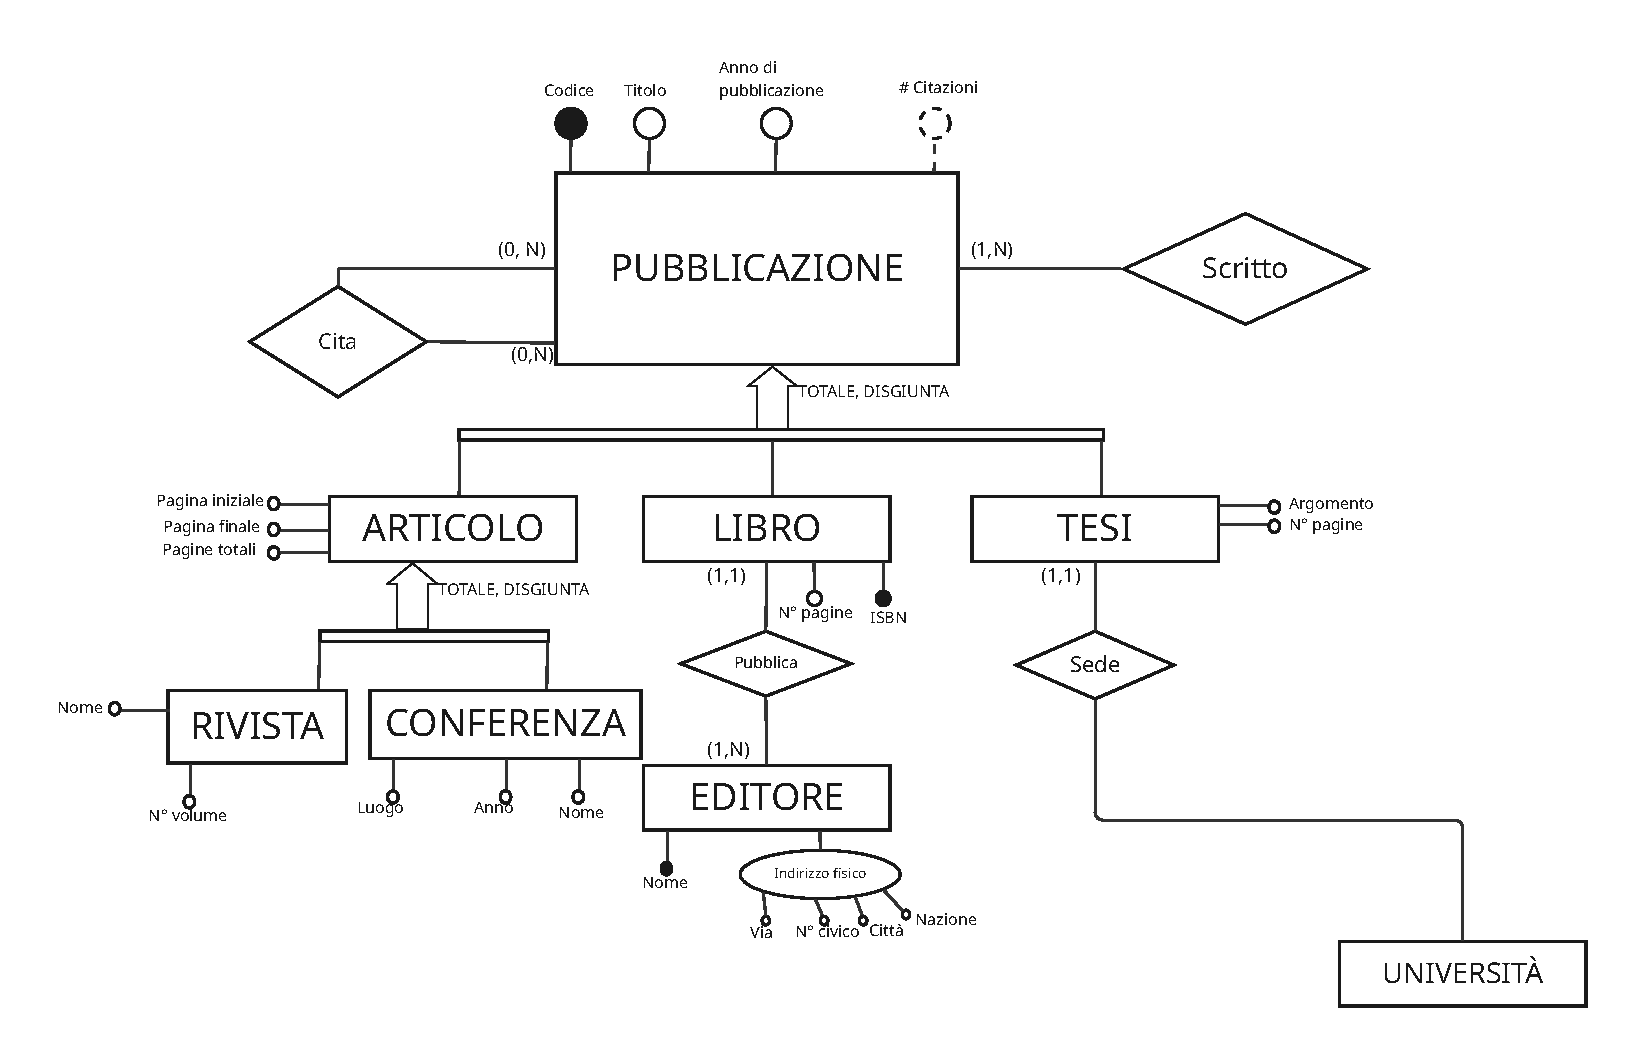
\includegraphics[width=0.8\textwidth]{img/EntitaPubblicazione.pdf} % image file path
    \caption{Entità Pubblicazione e specializzazioni}
    \label{fig:label_immagine}
\end{figure}
The entity \textbf{Publication} has been modeled as a parent entity with three specializations: \textbf{Journal Article}, \textbf{Book}, and \textbf{Thesis}. This choice is motivated by the need to represent clearly and structurally the differences between the various types of publication, which have specific attributes and distinct relationships with other entities (for example, the publisher for books and the university for theses). The specialization has been implemented using a total coverage hierarchy, where each publication must necessarily be classified as one of the three specific types. The entity \textbf{Journal Article} is further specialized into \textbf{Journal} and \textbf{Conference}, as they manage distinct attributes (for example, the volume number for journals and the conference location for conference papers). The specialization is total disjoint, as they cover all articles but do not overlap with each other.
The entity \textbf{Publisher} is linked to the entity \textbf{Book} through a publication relationship, and presents a composite attribute \textit{Address} that includes street, house number, city, and country. The relationship is one to many, as a publisher can publish multiple books. Finally, as written above, citations are managed as a recursive relationship between publications, allowing for an effective modeling of the bibliographic reference dynamics within the system.
\\We assume that the name of the publisher is unique within the domain, given the regional context to which we refer.

\subsection{Management of the Affiliation Entity and Its Specializations} \label{subsec:affiliazione}
\begin{figure}[H]
    \centering
    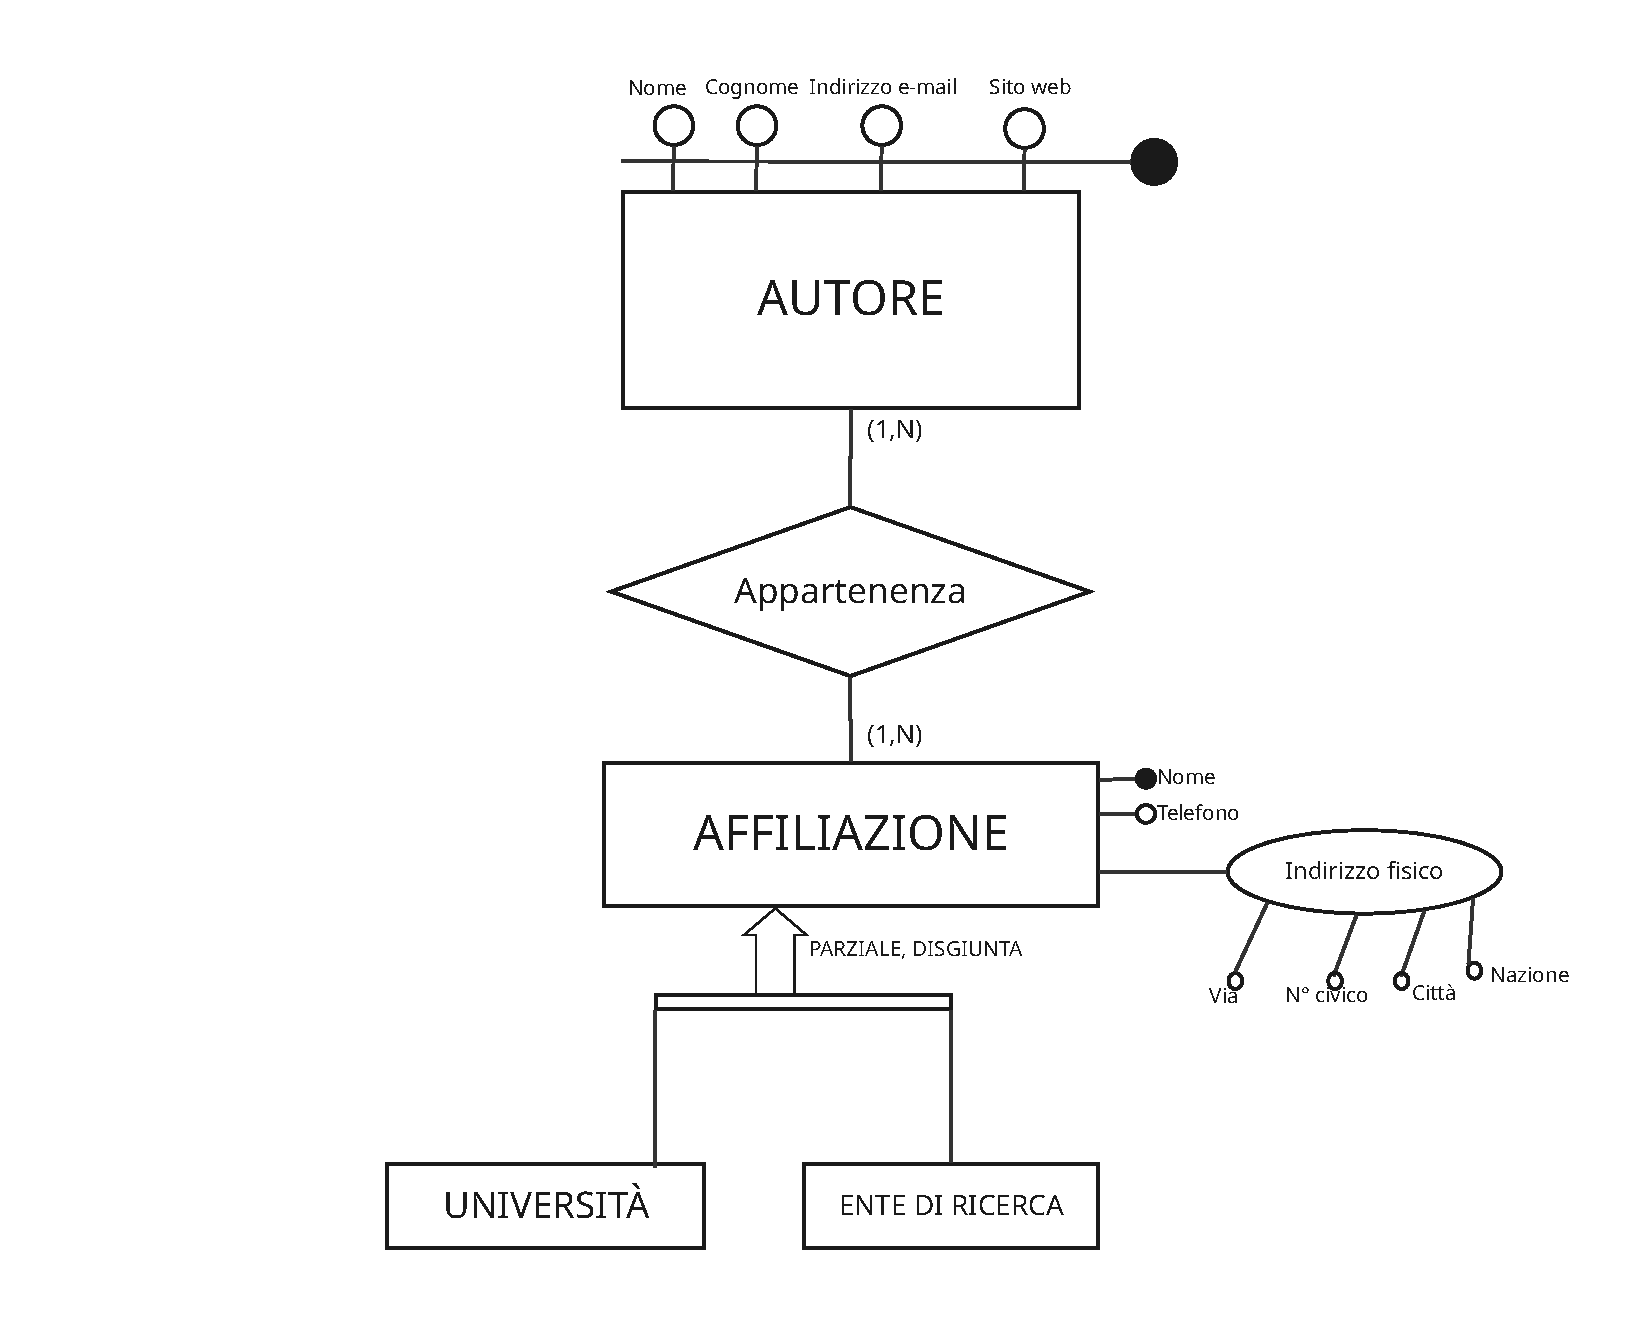
\includegraphics[width=0.8\textwidth]{img/EntitaAutore.pdf} % image file path
    \caption{Author, Affiliation and specializations entity}
    \label{fig:label_immagine}
\end{figure}
The entity \textbf{Affiliation} has been specialized into \textbf{University} and \textbf{Research Institution} to represent more detailed the different types of affiliations that an author can have. This specialization has been implemented using a partial coverage hierarchy, as there may be affiliations that do not fall into either of the two categories. The choice to keep the child entities separate is motivated by the possibility of later linking the university to theses, while research institutions do not have this relationship. The entity \textbf{Author} is linked to the entity \textbf{Affiliation} through a membership relationship, which allows modeling the fact that an author can be affiliated with multiple institutions over time. The relationship is many to many, as an author can have multiple affiliations and an affiliation can be associated with multiple authors. It is not required to manage the periods of membership from an author to an affiliation (historical tracking), for example if an author was affiliated with an affiliation in different periods, it is not necessary to keep track of this information.
\\As stated for the publisher, we assume that the name of the affiliation is unique within the domain, given the regional context to which we refer.
\\Note that the entity \textbf{Research Institution} has been added upon the instructor's suggestion, in order to represent more comprehensively the domain of affiliations, which are not limited exclusively to universities, but also include other types of organizations involved in academic research.
\\The entity \textbf{Author} presents a candidate key, composed by the \textbf{superkey}, as it is not specified by the requirements that any combination of attributes could serve as a unique identifier. 

\subsection{Integration of Components and Final Schema} \label{subsec:integrazione}
\begin{figure}[H]
    \centering
    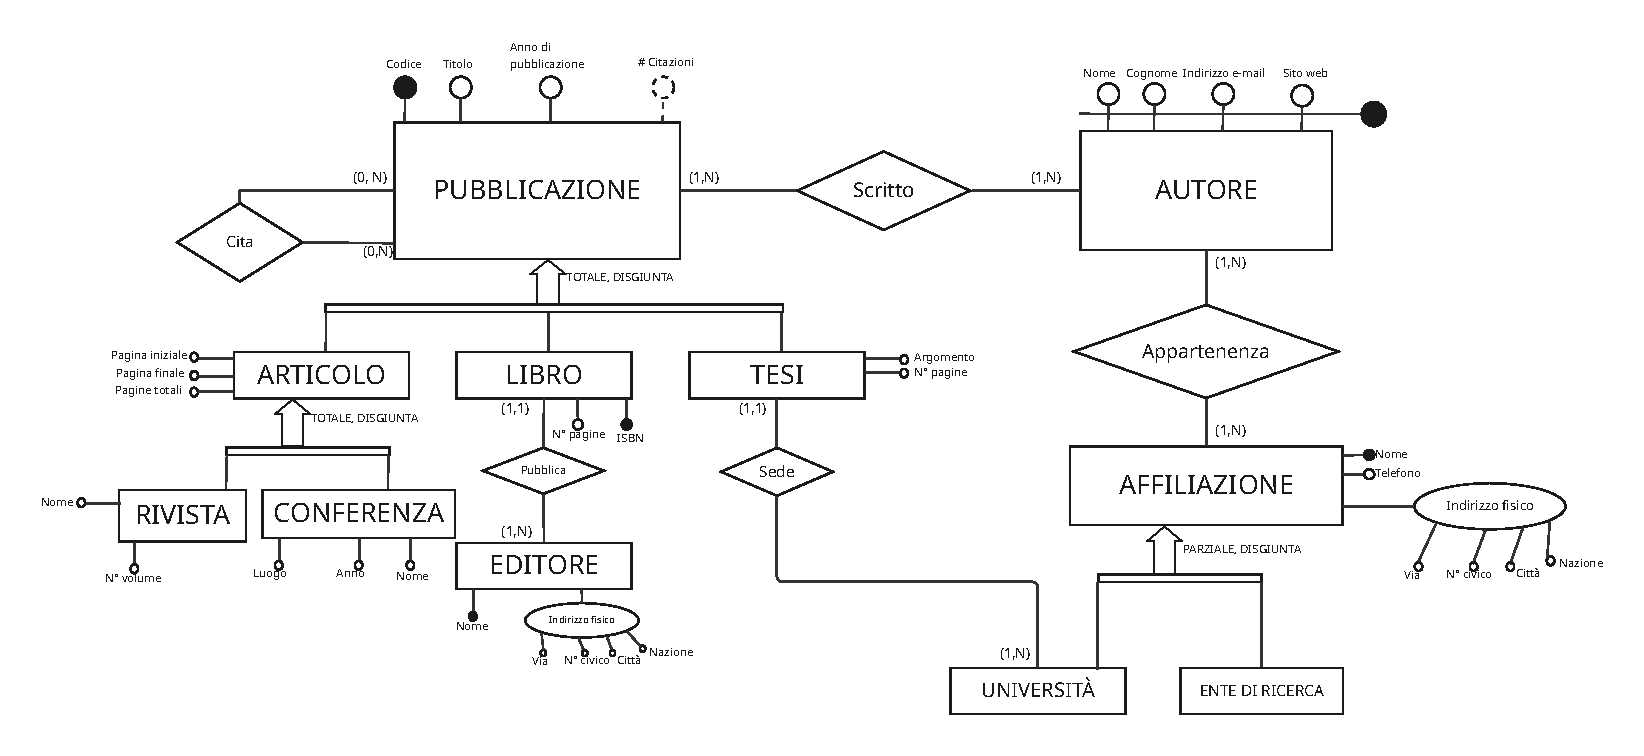
\includegraphics[width=0.8\textwidth]{img/EntitaRelazione.pdf} % image file path
    \caption{Entity-Relationship Schema}
    \label{fig:label_immagine}
\end{figure}
To integrate the produced components, a many-to-many relationship is created between \textbf{Author} and \textbf{Publication}. Finally, the entity \textbf{Thesis} is connected to the entity \textbf{University} through a defense relationship, since each thesis is defended at a specific university. This creates a problematic cycle, which is handled in later phases because it could lead to data inconsistencies. For example, an author affiliated with a research institution cannot be associated with a thesis, but if the cycle is not managed, they could be linked to a thesis without having co-authors affiliated with the university where the thesis is defended.
\\ Some constraints cannot be resolved through the ER schema. For example, the no self-citation constraint (a publication cannot cite itself) or the acyclicity constraint (if B cites A, A cannot cite B) for citations cannot be managed at the conceptual design level, but it will be necessary to implement triggers at the physical design level to guarantee data integrity in these specific cases.
\section{Logical Design} \label{sec:progettazione-logica}
\subsection{Volume Table} \label{subsec:tavola-volumi}

\begin{tabularx}{\textwidth}{X X X}
\toprule
\textbf{Concept} & \textbf{Type} & \textbf{Volume} \\
\midrule
Publication & E & 100.000 \\
Journal article & E & 20.000 \\
Conference paper & E & 15.000 \\
Book & E & 10.000 \\
Thesis & E & 55.000 \\
Author & E & 70.000 \\
Affiliation & E & 200 \\
Publisher & E & 150 \\
University & E & 35 \\
Research institution & E & 100 \\
\midrule
Citation & R & 2.000.000 ($100.000 \times 20$) \\
Written & R & 330.000 ($3,3 \times 100.000$) \\
Membership & R & 140.000 ($70.000 \times 2$) \\
Defense & R & 55.000 \\
Publishes & R & 10.000 \\
\bottomrule
\end{tabularx}

\medskip

The volume table represents the fundamental step from conceptual design to logical design, providing a quantitative estimate of the load the database will have to support. The system manages a total of \textbf{100,000 publications}. Note how the sum of the child entities (\textit{Journal article, Conference paper, Book, Thesis}) is exactly 100,000, reflecting the choice of a \textbf{total coverage hierarchy}. Theses represent the largest share (55,000), consistent with an academic domain.

With \textbf{70,000 authors} and an average of 3.3 authors per publication (relationship \texttt{Written}), the system must manage about 330,000 author-publication links. The \texttt{Membership} relationship ($70.000 \times 2$) correctly models academic turnover, assuming that each author is affiliated with two different institutions over time.
The small number of \textbf{Affiliations (200)}, \textbf{Publishers (150)} and \textbf{Universities (35)} suggests that these tables will act as "control registries", with a low update rate compared to the transactional tables of publications and citations. In general, these volumes are suitable for a regional context, as hypothesized. Since there can be \textbf{Affiliations} that are neither \textbf{Universities} nor \textbf{Research Institutions}, we estimated 65 affiliations that do not fall into either category, bringing the total to 200.
The estimate of 20 citations per publication was made considering that there may be many publications with another degree of internal self-reference within our context.
\subsection{Redundancy Analysis} \label{subsec:analisi-ridondanze}
\subsubsection*{Frequency of the Most Common Operations}
Here is an estimate of the frequency of the most common operations the system will have to handle, based on reasonable assumptions consistent with the regional academic domain:
\begin{enumerate}[label=\textbf{OP\arabic*}, start=1, leftmargin=1.5cm]
    \item \textbf{Publication printing} \\
    Frequency: 500 times per day.
    
    \item \textbf{Publication insertion} \\
    Insert a publication (40 times per day). \\
    \item \textbf{Insert an author} \\
    Frequency: 10 times per day.
    \item \textbf{Modify affiliation} \\
    Frequency: 1 time per day (estimated frequency).
\end{enumerate}
\subsubsection{Redundant Attributes}
The only redundant attribute present in the schema is \texttt{NumeroCitazioni} in the \textbf{Publication} entity. A comparative analysis is made between the two solutions for the attribute, considering the impact of redundancy on system efficiency, particularly for the printing and citation update operations, which are the most frequent. In the redundancy analysis, only operations 1 and 2 are considered because they involve the \textbf{Publication} entity and the redundant attribute \texttt{NumeroCitazioni}, while operations 3 and 4 do not directly involve this attribute.
\subsubsection{With Redundancy of the NumeroCitazioni Attribute} 
For the cost calculation, it is assumed that an access to an entity or relationship of type "L" (read) has a unit cost of 1, while an access of type "S" (write) has a unit cost of 2 \textit{(ratio 1:2)}, reflecting the additional overhead associated with write operations compared to reads. 
The total cost estimate is made using the higher frequency data for each operation, in order to evaluate the maximum impact of redundancy on system efficiency.
\subsubsection*{Operation 1}
\begin{tabular}{llll}
\toprule
\textbf{Concept} & \textbf{Construct} & \textbf{Accesses} & \textbf{Type} \\
\midrule
Publication & Entity & 1 & L \\
\bottomrule
\end{tabular}

\medskip
\textbf{Cost:} $(500 \times 1) \times 1 = 500$ units/day

\subsubsection*{Operation 2}
\begin{tabular}{llll}
\toprule
\textbf{Concept} & \textbf{Construct} & \textbf{Accesses} & \textbf{Type} \\
\midrule
Publication & Entity & 2 & S \\
Citation          & Relationship & 1 & S \\
Publication & Entity & 1 & L \\
Written        & Relationship & 1 & S \\
\bottomrule
\end{tabular}

\paragraph{Logical steps:}
\begin{enumerate}[label=\textbf{\arabic*)}, start=1, leftmargin=1.5cm]
    \item Save the publication data
    \item Save the publication and cited publication pairs
    \item Find the cited publication
    \item Increment that publication's number of citations by 1
    \item Save the publication-author pair
\end{enumerate}

\textbf{Cost:} $(40 \times 4) \times 2 + (40 \times 1) \times 1 = 360$ units/day

\subsubsection{Without Redundancy of the NumeroCitazioni Attribute} 

\subsubsection*{Operation 1}
\begin{tabular}{llll}
\toprule
\textbf{Concept} & \textbf{Construct} & \textbf{Accesses} & \textbf{Type} \\
\midrule
Publication & Entity    & 1  & L \\
Citation     & Relationship & 20 & L \\
\bottomrule
\end{tabular}

\paragraph{Description:} 
I print the data related to a publication. For each publication, to calculate the number of citations I access the Citation relationship. The average number of accesses per Publication is calculated as: $\frac{\text{Citation volume}}{\text{Publication volume}} = 20$.

\medskip
\textbf{Cost:} $500 \times (20 + 1) \times 1 = 10.500$ units/day

\subsubsection*{Operation 2}
\begin{tabular}{llll}
\toprule
\textbf{Concept} & \textbf{Construct} & \textbf{Accesses} & \textbf{Type} \\
\midrule
Publication & Entity & 1 & S \\
Citation          & Relationship & 1 & S \\
Written        & Relationship & 1 & S \\
\bottomrule
\end{tabular}

\paragraph{Logical steps:}
\begin{enumerate}[label=\textbf{\arabic*)}, start=1, leftmargin=1.5cm]
    \item Save the publication data
    \item Save the pairs of publication and cited publication
    \item Save the publication-author pair
\end{enumerate}

\medskip
\textbf{Cost:} $40 \times 3 \times 2 = 240$ units/day

\subsubsection{Comparative Study} 

\begin{table}[h]
\centering
\begin{tabular}{lcc}
\toprule
\textbf{Cost} & \textbf{With redundancy} & \textbf{Without redundancy} \\
\midrule
OP1 & 500 & 10.500 \\
OP2 & 360 & 240 \\
\midrule
\textbf{Total} & \textbf{860} & \textbf{10.740} \\
\bottomrule
\end{tabular}
\end{table}

\textbf{Conclusion:} Since $860 < 10.740$, it is convenient to keep the derived attribute.

\subsection{ER schema restructuring} \label{subsec:ristrutturazione-schema}
The following shows the changes made to the ER model to facilitate translation to the relational logical schema, with particular attention to handling specializations and simplifying some complex structures.

\begin{figure}[H]
    \centering
    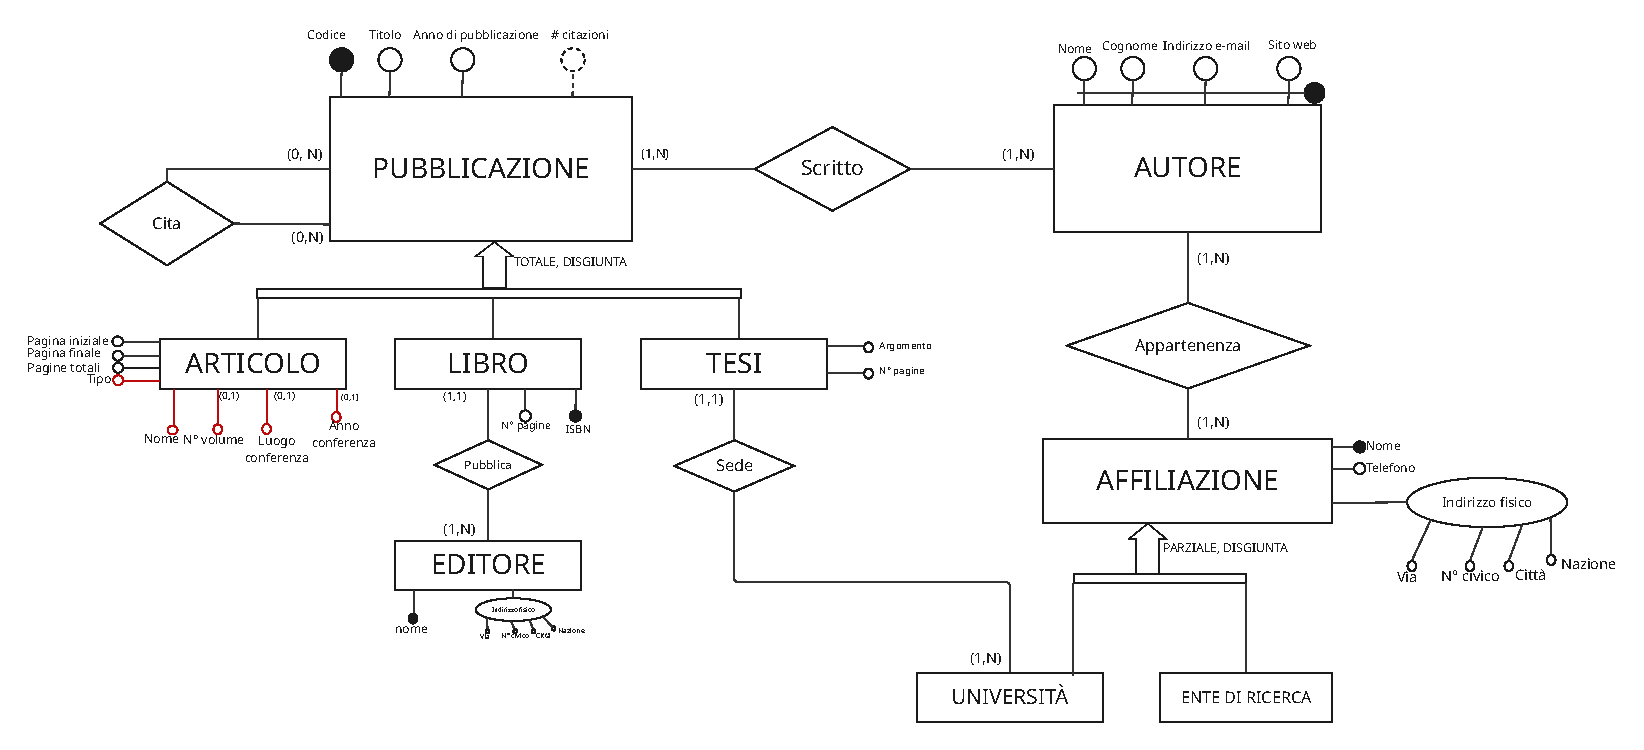
\includegraphics[width=0.8\textwidth]{img/ER1.pdf} % image file path
    \caption{ER schema modified after the first revision}
    \label{fig:label_immagine2}
\end{figure}
\noindent
\textbf{Journal-Conference Specialization:} 
The hierarchy was merged upward (restructuring toward the parent) by removing the child entities and migrating their attributes into the parent entity \textit{Article}. To distinguish occurrences, the discriminating attribute \textit{Type} was introduced, with values constrained to the domain $\{\text{Journal, Conference}\}$. 

The attributes inherited from the child entities were defined as optional (cardinality 0,1), with the exception of the attribute \textit{Name}, which remains mandatory because it is common to both types. It is also specified that the attribute \textit{ConferenceYear} must be semantically distinct from the attribute \textit{PublicationYear}. For example, a conference can be held in a different year than the publication year of the associated article.

\begin{figure}[H]
    \centering
    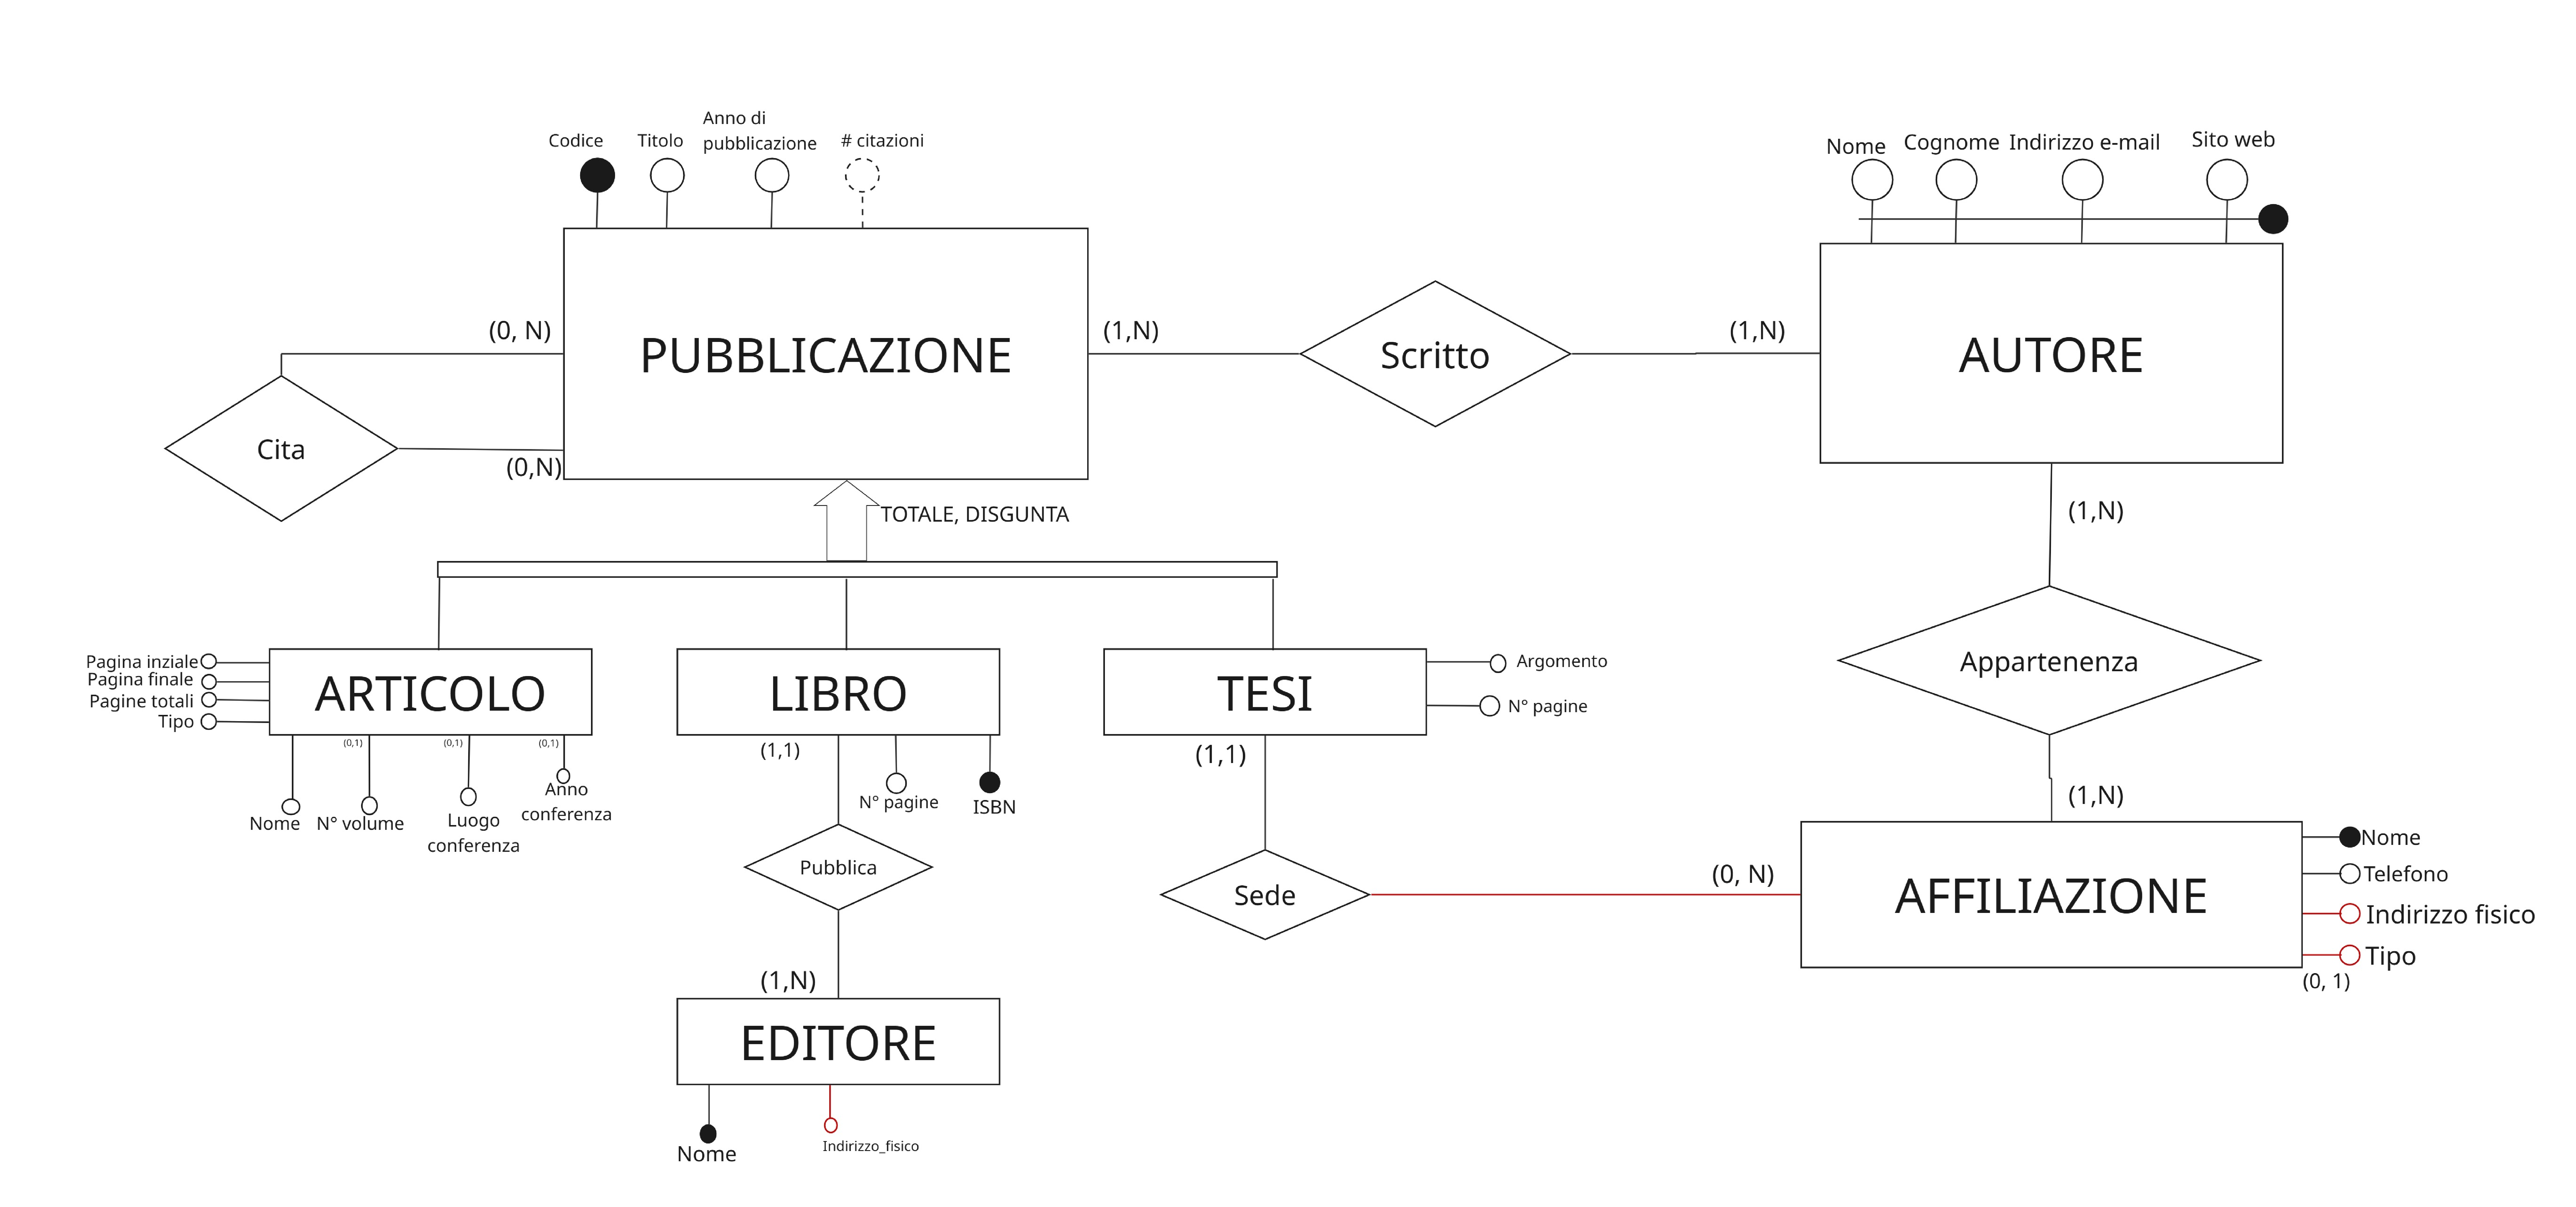
\includegraphics[width=0.8\textwidth]{img/ER2.pdf} % image file path
    \caption{ER schema modified after the second revision}
    \label{fig:label_immagine3}
\end{figure}

\noindent
\textbf{Affiliation Hierarchy Simplification:}
The specialization between the entity \textit{Affiliation} (parent) and the subentities \textit{University} and \textit{ResearchInstitute} was resolved by merging upward to the parent. This choice is motivated by the absence of relevant specific attributes in the child entities. 

To preserve the original semantics, an integrity constraint based on the affiliation type was introduced: association with the entity \textit{Thesis} is valid exclusively for occurrences of type \textit{University}. In terms of cardinality, the relationship between \textit{Thesis} and \textit{Affiliation} is $(1,1)$, while the participation of the entity \textit{Affiliation} is $(0,n)$, because only the subset related to universities can be associated with a thesis.

\noindent
\textbf{Address Attribute Simplification:}
The composite attribute \textit{PhysicalAddress} was restructured by aggregating its components (such as street, street number, postal code and city). To simplify implementation in the logical model and facilitate insert operations, the individual fields were unified into a single atomic string attribute. This is done because composite attributes do not exist in the relational logical model, so it is necessary to simplify the attribute structure to ensure a more direct translation without loss of information.

\begin{figure}[H]
    \centering
    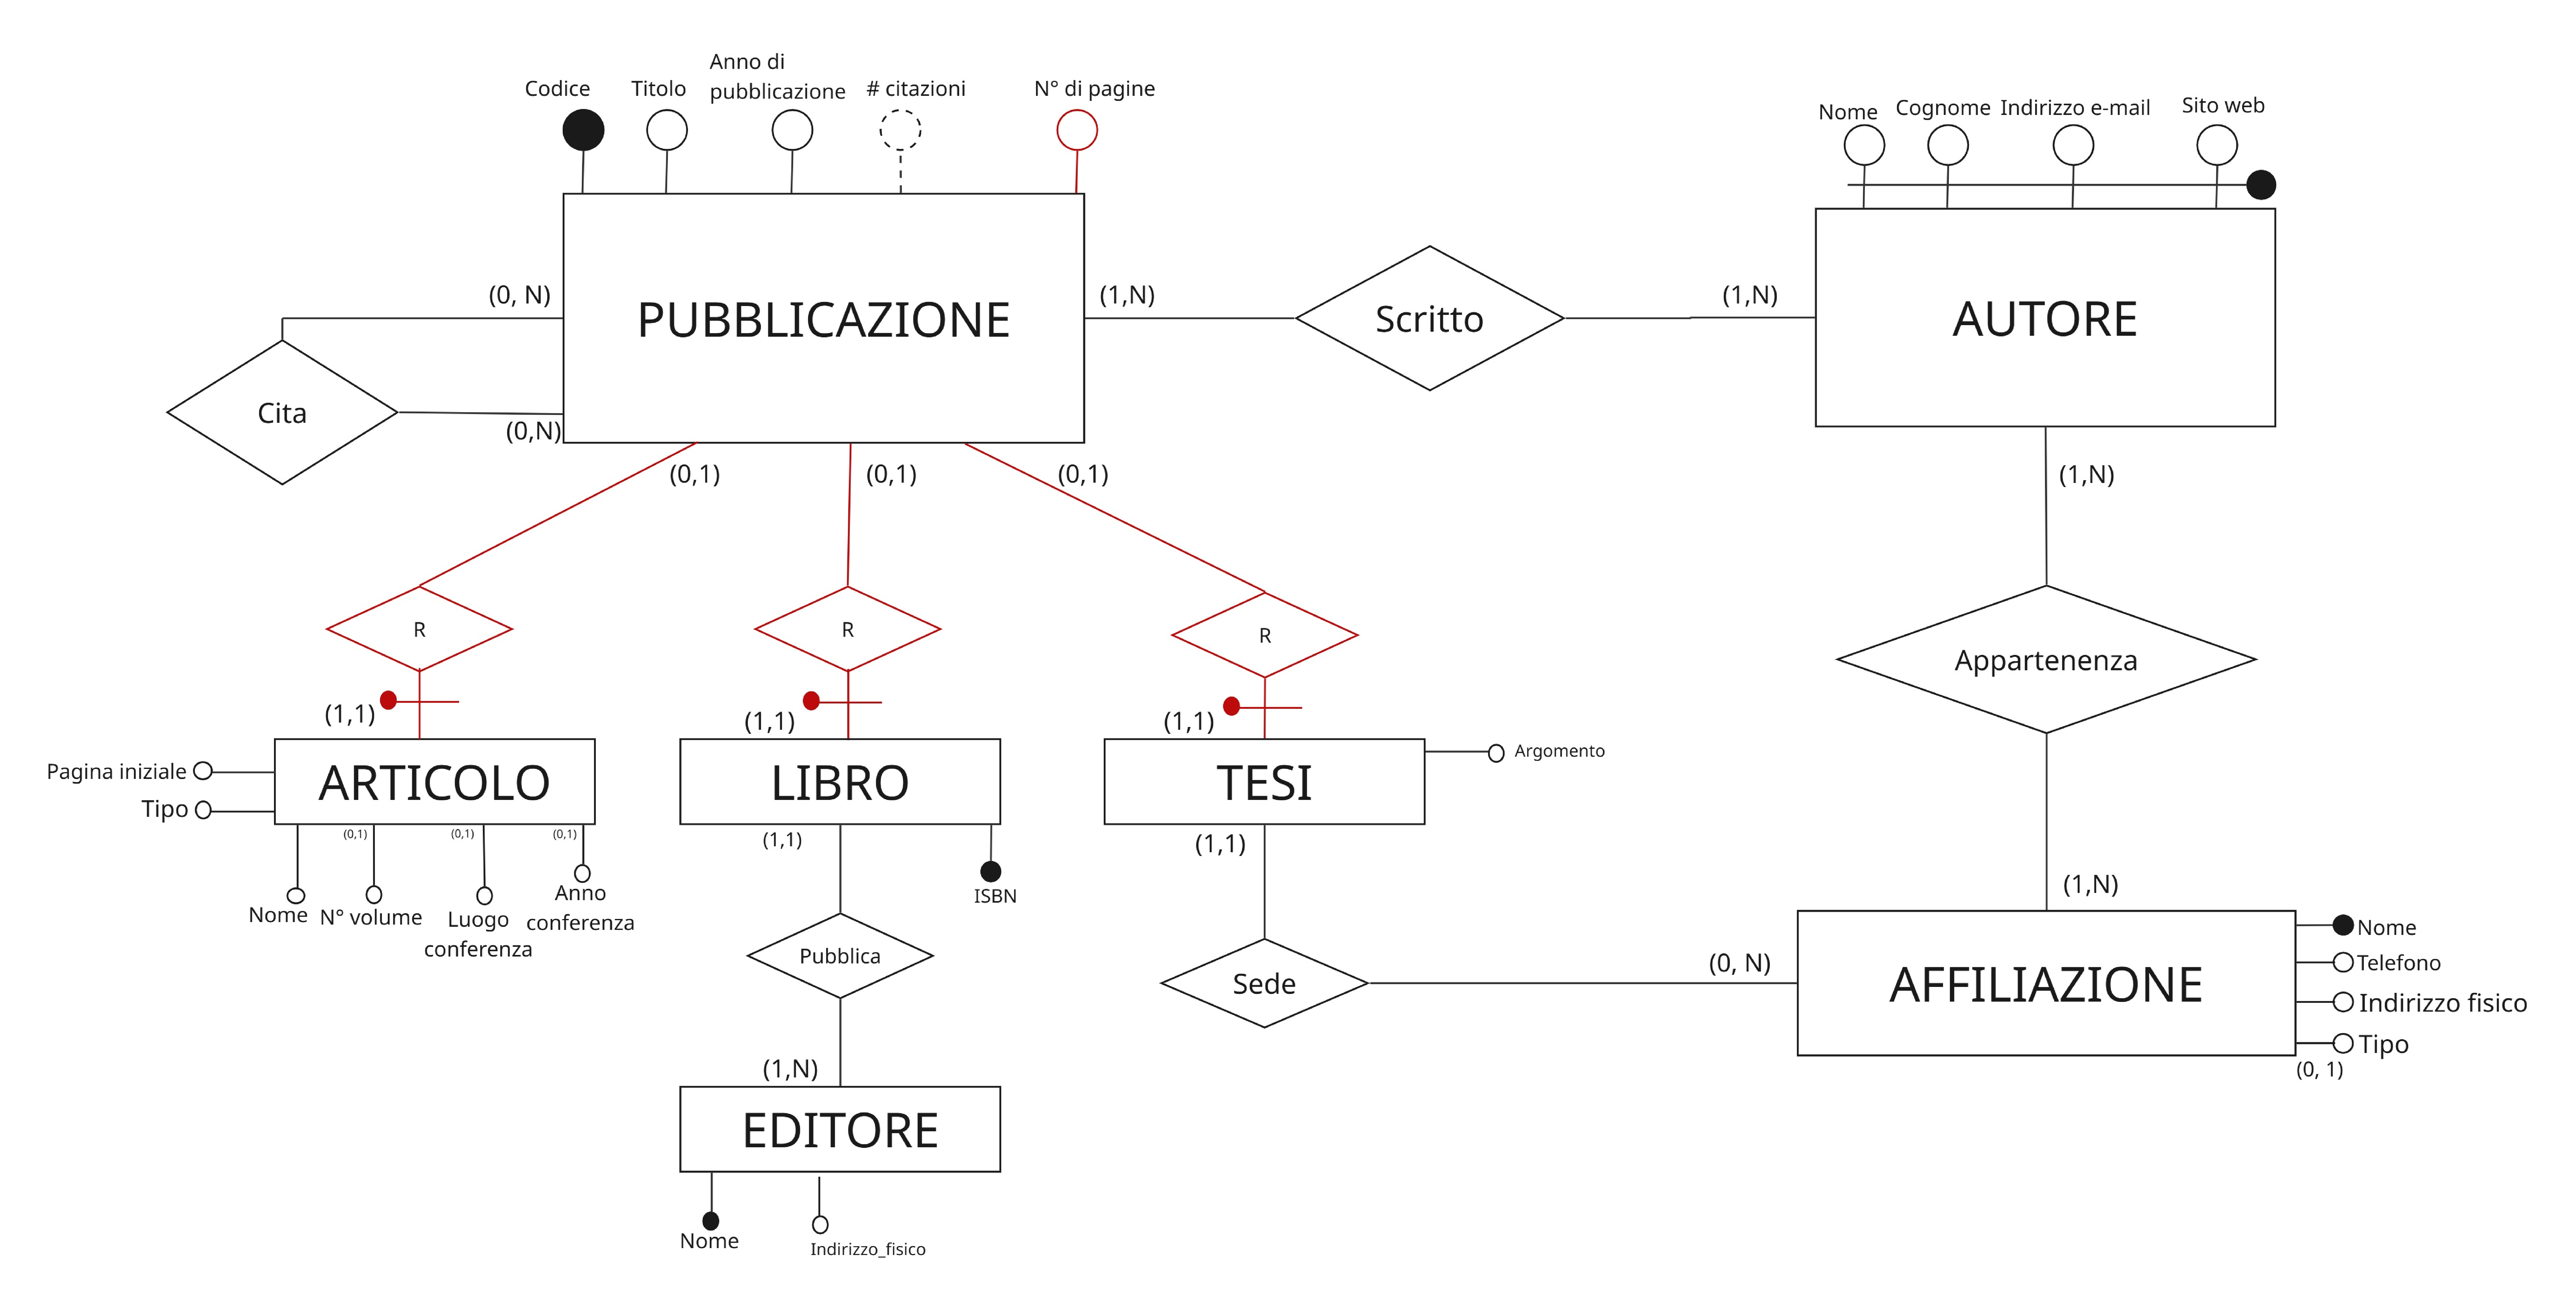
\includegraphics[width=0.8\textwidth]{img/ER3.pdf} % image file path
    \caption{ER schema modified after the third revision}
    \label{fig:label_immagine4}
\end{figure}

\noindent
\textbf{Publication Hierarchy Resolution:}
The specialization between the parent entity \textit{Publication} and the subentities \textit{Article}, \textit{Book} and \textit{Thesis} was resolved by keeping the entities distinct (multiple entity strategy). 

To correctly implement the logical link, explicit relationships between the parent and the children were defined via foreign keys in the child entities referencing the primary key of \textit{Publication}. To ensure total coverage of the specialization, an additional integrity constraint was introduced: each occurrence of the entity \textit{Publication} must necessarily be referenced as a foreign key in at least one of the three child entities.
\\ \textbf{Page attribute simplifications:} Since \texttt{TotalPageCount} is a common attribute to all the subentities of the entity \textbf{Publication}, it was moved to the parent entity. From there, it was decided to remove the attribute \texttt{EndPage} from \textbf{Article}, since it can be easily calculated from \texttt{StartPage} and \texttt{TotalPageCount}. 
\begin{figure}[H]
    \centering
    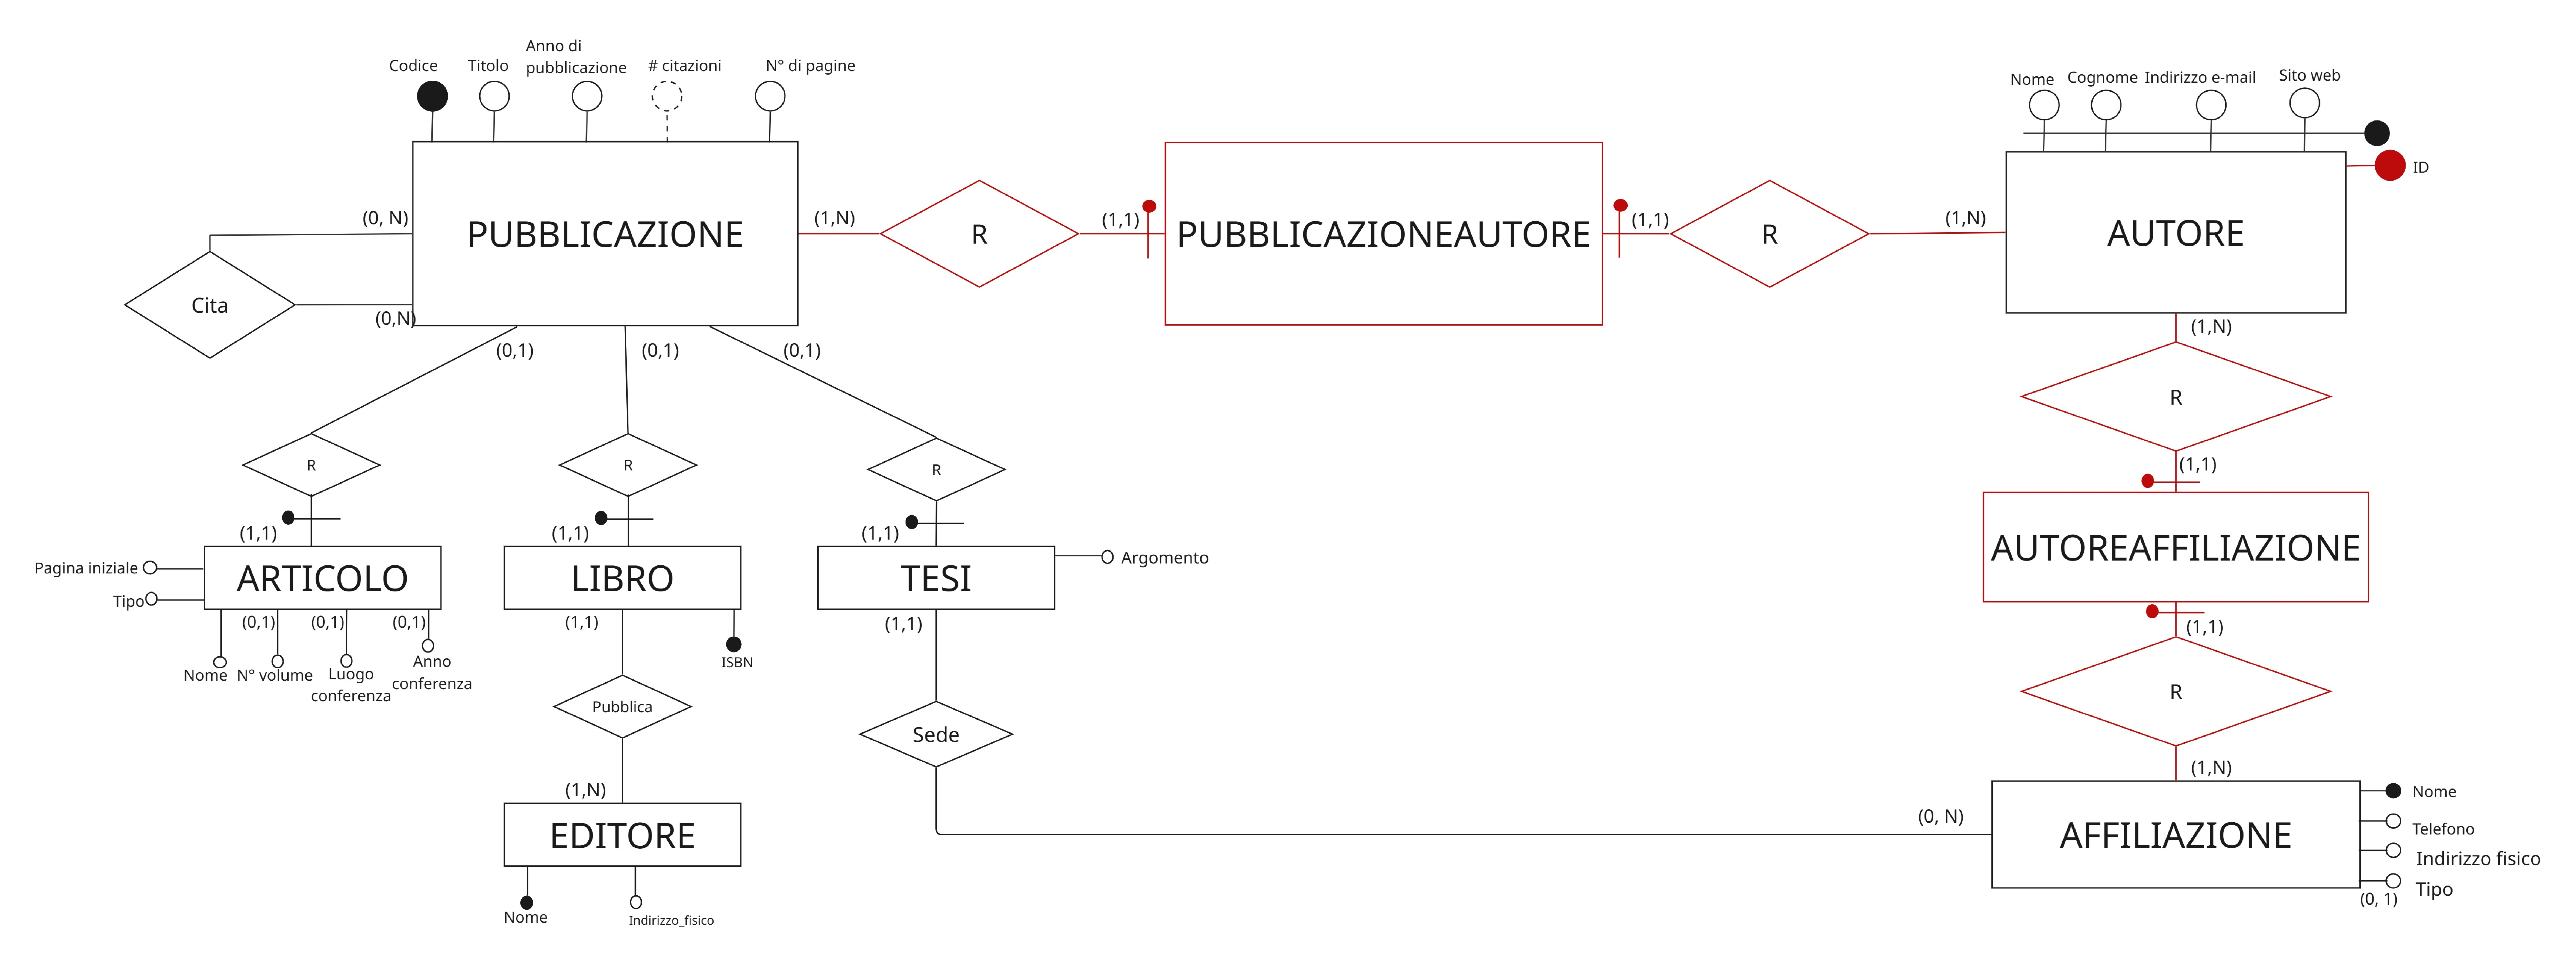
\includegraphics[width=0.8\textwidth]{img/ER4.pdf} % image file path
    \caption{ER schema modified after the fourth revision}
    \label{fig:label_immagine5}
\end{figure}

\noindent
\textbf{"Written" and "Membership" relationship restructuring, key on Author:}
The relationship \textbf{Written} was restructured by introducing an associative entity called \textbf{PublicationsAuthors}, which links the entity \textbf{Author} with the entity \textbf{Publication}. This choice is motivated by the need to correctly represent the many-to-many relationship between authors and publications, allowing effective management of cases where a publication has multiple authors and an author has multiple publications. The same approach was adopted for the \textit{Membership} relationship, with the introduction of the associative entity \textbf{AuthorAffiliation} linking the entity \textbf{Author} with the entity \textbf{Affiliation}. This restructuring makes it possible to model the affiliation dynamics of authors more flexibly, as they can be associated with multiple organizations over time, and to maintain clear traceability of relationships between authors and affiliations.
\\ Finally, it was noted that the entity \textbf{Author} has only a superkey, since the requirements do not specify that any attribute can act as a unique identifier. Therefore, a new attribute \textit{ID} was introduced as a candidate key for the entity \textbf{Author}, thus ensuring uniqueness.

\begin{figure}[h]
    \centering
    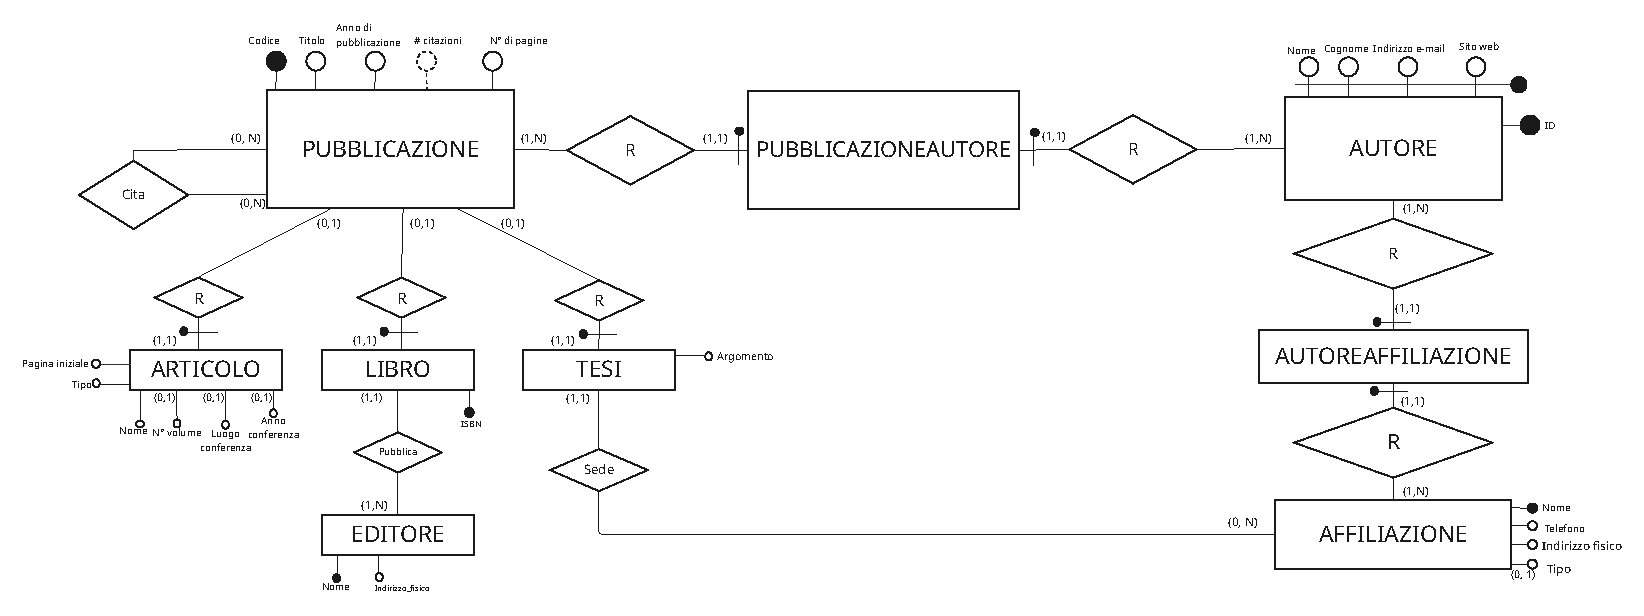
\includegraphics[width=0.8\textwidth]{img/ER5.pdf} % image file path
    \caption{Final ER schema without detailed modifications}
    \label{fig:label_immagine}
\end{figure}
It should be noted that the ER model cannot handle the non-self-citation and non-circular-citation constraints. The problematic cycle created by the relationship between \textit{Publication}, \textit{Author} and \textit{Affiliation} is also not manageable. These constraints will be handled at the physical design level, through the implementation of triggers that ensure data consistency during insert and update operations.
\subsection{Logical schema} \label{subsec:schema-relazionale}

From the final ER model, the following relational logical schema is obtained:
\\PUBLICATIONS(\underline{Code},Title, Year, PageCount, CitationCount) \\
ARTICLES(\underline{PublicationCode}, Name, VolumeNumber, ConferenceLocation, ConferenceYear, StartPage, Type) \\
BOOKS(\underline{PublicationCode}, ISBN, PublisherName) \\
THESES(\underline{PublicationCode}, Topic, Affiliation) \\
AUTHORS(\underline{ID}, Name, Surname, Email, Website) \\
AFFILIATIONS(\underline{Name}, Address, Phone, Type) \\
PUBLISHERS(\underline{Name}, Address) \\
CITATIONS(\underline{CitingPublication}, \underline{CitedPublication}) \\
PUBLICATIONAUTHOR(\underline{AuthorID}, \underline{PublicationCode}) \\
AUTHORAFFILIATION(\underline{AuthorID}, \underline{AffiliationName}) \\
*primary keys are underlined, while foreign keys are indicated with arrows.

\textbf{Foreign keys:} \\
$\text{ARTICOLI.CodicePubblicazione} \rightarrow \text{PUBBLICAZIONI.Codice}$ \\
$\text{LIBRI.CodicePubblicazione} \rightarrow \text{PUBBLICAZIONI.Codice}$ \\
$\text{TESI.CodicePubblicazione} \rightarrow \text{PUBBLICAZIONI.Codice}$ \\
$\text{CITAZIONI.PubblicazioneCitante} \rightarrow \text{PUBBLICAZIONI.Codice}$ \\
$\text{CITAZIONI.PubblicazioneCitata} \rightarrow \text{PUBBLICAZIONI.Codice}$ \\
$\text{LIBRI.NomeEditore} \rightarrow \text{EDITORI.Nome}$ \\
$\text{TESI.Affiliazione} \rightarrow \text{AFFILIAZIONI.Nome}$ \\
$\text{PUBBLICAZIONEAUTORE.IDAutore} \rightarrow \text{AUTORI.ID}$ \\
$\text{PUBBLICAZIONEAUTORE.CodicePubblicazione} \rightarrow \text{PUBBLICAZIONI.Codice}$ \\
$\text{AUTOREAFFILIAZIONE.IDAutore} \rightarrow \text{AUTORI.ID}$ \\
$\text{AUTOREAFFILIAZIONE.NomeAffiliazione} \rightarrow \text{AFFILIAZIONI.Nome}$ \\
\\
Note that primary keys were defined to guarantee the uniqueness of each record, while foreign keys were implemented to maintain referential integrity between tables, ensuring that the logical relationships between data are respected. The only candidate key not chosen as the primary key is ISBN in the \textbf{LIBRI} table, because the publication code is already a unique identifier sufficient to distinguish every book in the system. A single primary key was preferred to simplify join operations and reduce model complexity, avoiding the need to manage composite or multiple keys for the same entity. \\
Finally, the PK of \textbf{AUTORE} is an artificial primary key, since it is much more intuitive and faster than managing a composite key consisting of multiple attributes (e.g. name, surname, email).
\subsubsection*{Constraints not managed by the logical schema} 
The constraints not managed by the logical schema are:
\begin{itemize}
    \item Non self-citation: a publication cannot cite itself.
    \item Non circular citation: if publication A cites publication B, then publication B cannot cite publication A.
    \item Problematic cycle between Publication, Author and Affiliation: an author affiliated with a research institute cannot be associated with a thesis, but if the cycle is not managed they could be associated with a thesis without having co-authors affiliated with the university where the thesis is hosted.
    \item Total coverage constraint for the Publication-Article/Book/Thesis specialization: every publication must necessarily be classified as one of the three specific types.
    \item Integrity constraint for the Affiliation-University/Research Institute specialization: association with the Thesis entity is valid exclusively for occurrences of type University.
    \item Domain constraint for the Type attribute in Article: values must be constrained to the domain {Rivista, Conferenza}.
    \item Integrity constraint for Article attributes: the attributes NumeroVolume, LuogoConferenza and AnnoConferenza must be filled only if Type is Conferenza, while the attribute PaginaIniziale must be filled only if Type is Rivista.
\end{itemize} 
The most interesting constraints will be implemented at the physical design level through triggers.

\section{Physical design (DB implementation)} \label{sec:progettazione-fisica}
The DB was implemented using the PostgreSQL relational database management system, chosen for its robustness, scalability and advanced support for the functionalities required by the project. The physical design followed best practices for performance optimization, data integrity management and maintainability. The following sections describe the main implementation phases, including SQL table generation, database population with sample data and trigger implementation to ensure data consistency.
\subsection{SQL Table Generation}
Below is the SQL syntax used to create the database tables, in Data Definition Language (DDL). The table definitions include the specification of primary keys, foreign keys, and integrity constraints to ensure data consistency and compliance with the logical relationships between entities.

\begin{lstlisting}

-- Tabella Affiliazioni
CREATE TABLE affiliazioni
(
    nome varchar(100) NOT NULL ,
    telefono varchar(100) NOT NULL ,
    indirizzo varchar(100) NOT NULL ,
    tipo varchar(20),
    CONSTRAINT affiliazione_pkey PRIMARY KEY ( nome )
);

-- Tabella Pubblicazioni
CREATE TABLE pubblicazioni
(
    codice SERIAL NOT NULL,
    titolo varchar(200),
    annopubblicazione integer NOT NULL,
    ncitazioni integer CHECK( ncitazioni >= 0) DEFAULT 0 ,
    npagine integer CHECK( npagine > 0) NOT NULL ,
    CONSTRAINT pubblicazione_pkey PRIMARY KEY (codice)
);

-- Tabella Articoli
CREATE TABLE articoli(
    CodicePubblicazione integer NOT NULL,
    tipo varchar(50) NOT NULL CHECK(tipo IN ('Rivista', 'Conferenza')),
    nome varchar(255) NOT NULL,
    Npaginainiziale integer,
    Nvolume integer,
    luogoConferenza varchar(100),
    annoConferenza integer,
    CONSTRAINT articolo_pkey PRIMARY KEY (CodicePubblicazione),
    CONSTRAINT articolo_codice_pubblicazione_fkey FOREIGN KEY (CodicePubblicazione)
    REFERENCES public.pubblicazioni(codice) MATCH SIMPLE
    ON UPDATE NO ACTION
    ON DELETE CASCADE
);

-- Tabella AutoreAffiliazione
CREATE TABLE autoreaffiliazione
(
    idAutore integer NOT NULL,
    nomeAffiliazione varchar(255) NOT NULL,
    CONSTRAINT autoreaffiliazione_pkey PRIMARY KEY (idautore,nomeaffiliazione),
    CONSTRAINT auto_aff_id_autore_fkey FOREIGN KEY (idautore)
    REFERENCES public.autori(id) MATCH SIMPLE
    ON UPDATE CASCADE
    ON DELETE CASCADE,
    CONSTRAINT auto_aff_nome_affiliazione_fkey FOREIGN KEY(nomeaffiliazione)
    REFERENCES public.affiliazioni(nome) MATCH SIMPLE
    ON UPDATE CASCADE
    ON DELETE CASCADE
);

-- Tabella Autori
CREATE TABLE autori
(
    id SERIAL NOT NULL,
    nome varchar(100) NOT NULL,
    cognome varchar(100) NOT NULL,
    email varchar(100) NOT NULL,
    sitoweb varchar(100) NOT NULL,
    CONSTRAINT autore_pkey PRIMARY KEY(id)
);
-- Tabella Citazioni
CREATE TABLE citazioni
(
    pubblicazioneCitante integer NOT NULL ,
    pubblicazioneCitata integer NOT NULL ,
    CONSTRAINT citazione_pkey PRIMARY KEY (pubblicazioneCitante,pubblicazioneCitata),
    CONSTRAINT citazione_codice_pubblicazione_citante_fkey FOREIGN KEY (pubblicazioneCitante)
    REFERENCES public.pubblicazioni(codice) MATCH SIMPLE
    ON UPDATE NO ACTION
    ON DELETE CASCADE,
    CONSTRAINT citazione_codice_pubblicazione_citata_fkey FOREIGN KEY (pubblicazioneCitata)
    REFERENCES public.pubblicazioni(codice) MATCH SIMPLE
    ON UPDATE NO ACTION
    ON DELETE CASCADE
);
-- Tabella Editori
CREATE TABLE editori
(
    nome varchar(100) NOT NULL,
    indirizzo varchar(255) NOT NULL,
    CONSTRAINT editore_pkey PRIMARY KEY(nome)
);
-- Tabella Libri
CREATE TABLE libri
(
    CodicePubblicazione integer NOT NULL,
    isbn varchar(17) UNIQUE NOT NULL,
    nomeEditore varchar(100) NOT NULL,
    CONSTRAINT libro_pkey PRIMARY KEY (CodicePubblicazione),
    CONSTRAINT libro_codice_pubblicazione_fkey FOREIGN KEY (CodicePubblicazione)
    REFERENCES public.pubblicazioni(codice) MATCH SIMPLE
    ON UPDATE NO ACTION
    ON DELETE CASCADE,
    CONSTRAINT libro_nome_editore_fkey FOREIGN KEY (nomeEditore)
    REFERENCES public.editori(nome) MATCH SIMPLE
    ON UPDATE NO ACTION
    ON DELETE NO ACTION
);
-- Tabella PubblicazioneAutore
CREATE TABLE pubblicazioneautore
(
    CodicePubblicazione integer NOT NULL,
    idAutore integer NOT NULL,
    CONSTRAINT pubb_autore_pkey PRIMARY KEY (CodicePubblicazione,idAutore),
    CONSTRAINT pubb_autore_codice_pubblicazione_fkey FOREIGN KEY (CodicePubblicazione)
    REFERENCES public.pubblicazioni(codice) MATCH SIMPLE
    ON UPDATE NO ACTION
    ON DELETE CASCADE,
    CONSTRAINT pubb_autore_id_autore_fkey FOREIGN KEY (idAutore)
    REFERENCES public.autori(id) MATCH SIMPLE
    ON UPDATE NO ACTION
    ON DELETE CASCADE
);

-- Tabella Tesi
CREATE TABLE tesi
(
    CodicePubblicazione integer NOT NULL ,
    argomento text NOT NULL ,
    nomeAffiliazione varchar (255) NOT NULL ,
    CONSTRAINT tesi_pkey PRIMARY KEY ( CodicePubblicazione ) ,
    CONSTRAINT tesi_codice_pubblicazione_fkey FOREIGN KEY (CodicePubblicazione)
    REFERENCES public.pubblicazioni(codice) MATCH SIMPLE
    ON UPDATE NO ACTION
    ON DELETE CASCADE ,
    CONSTRAINT tesi_nome_affiliazione_fkey FOREIGN KEY (nomeAffiliazione)
    REFERENCES public.affiliazioni ( nome ) MATCH SIMPLE
    ON UPDATE NO ACTION
    ON DELETE NO ACTION
);
\end{lstlisting}

\subsection{Database Population} \label{subsec:popolamento}
In this phase, the insertion of structured data into our database is carried out. To optimize time, the process was implemented using AI prompts, which allowed the generation of consistent and representative data records for the regional academic domain, drastically reducing manual data entry time and minimizing the risk of syntax errors.
\\For data extraction and formatting, we used \textbf{Gemini 3.1 Pro}, an advanced artificial intelligence language model developed by Google, to generate consistent and representative records for the academic domain.
The population of the tables was limited to the Triveneto area (\textit{Veneto}, \textit{Trentino-Alto Adige}, \textit{Friuli-Venezia Giulia}).
This strategic choice was dictated by a key factor: Triveneto boasts a solid and historic presence of numerous activities, universities, and centers of research excellence.
Focusing the scope on this territory made it possible to test the effectiveness of the prompt and the robustness of the database architecture on a dataset consistent with the volumes estimated in the volume table.
\\ Here is an example of a table resulting from the database population:

% ============================================================
% AFFILIAZIONE
% ============================================================
\begin{table}[H]
\centering
\caption{Affiliazione}
\small
\begin{tabular}{llll}
\toprule
\multicolumn{4}{c}{\textbf{Affiliation}} \\
\midrule
\textbf{Name} & \textbf{Phone} & \textbf{Address} & \textbf{Type} \\
\midrule
Università degli Studi di Udine   & 0432-556111 & Via Palladio 8, Udine              & Università      \\
Università degli Studi di Trieste & 040-5587111 & Piazzale Europa 1, Trieste         & Università      \\
SISSA                             & 040-3787111 & Via Bonomea 265, Trieste           & Università      \\
Università degli Studi di Padova  & 049-8275111 & Via 8 Febbraio 2, Padova           & Università      \\
Università Ca' Foscari Venezia    & 041-2345111 & Dorsoduro 3246, Venezia            & Università      \\
Area Science Park                 & 040-3755111 & Padriciano 99, Trieste             & Ente di ricerca \\
OGS                               & 040-21401   & Borgo Grotta Gigante 42/C, Sgonico & Ente di ricerca \\
CRO Aviano                        & 0434-659111 & Via Franco Gallini 2, Aviano       & Ente di ricerca \\
Università degli Studi di Trento  & 0471-011000 & Via Calepina 14, Trento            & Università      \\
Libera Università di Bolzano      & 0471-011000 & Piazza Università 1, Bolzano       & Università  \\
Fondazione Bruno Kessler          & 0461-314200 & Via Santa Croce 77, Trento       & Ente di ricerca \\
\bottomrule
\end{tabular}
\end{table}


\subsection{Trigger} \label{subsec:trigger-citazioni}
At the instructor's request, we decided to implement the most interesting and relevant triggers for our domain, particularly those related to the management of citations.
\subsubsection*{Logical properties of citation constraints}
\textbf{Non Autocitazione}: Una pubblicazione non può citare sé stessa. Questo è il vincolo più elementare e serve a prevenire l'inserimento di dati logicamente inconsistenti, garantendo che il conteggio delle citazioni rifletta solo i riferimenti esterni.\\
\textbf{Non Citazione Circolare}: Una pubblicazione A non può citare una pubblicazione B se B cita già A, direttamente o indirettamente. Questo vincolo impedisce la formazione di cicli di citazione che potrebbero distorcere il conteggio delle citazioni e complicare l'analisi bibliometrica.\\
\textbf{Nota sul Vincolo Temporale}: Una pubblicazione non può citare un'altra pubblicazione con un anno di pubblicazione successivo. Pur riconoscendo l'esistenza di casi come i preprint nel mondo reale, questo vincolo è assunto logicamente come rilevante ed è implementato nel database.\\

\subsubsection{Trigger for incrementing the number of citations}
The trigger \texttt{inc\_n\_citazioni} is designed to handle the increment of the citation count for a publication whenever a new citation involving it is inserted. The trigger performs the following operations:
1. It checks that the citing publication is not the same as the cited publication, thus preventing self-citation.
2. It ensures that the citing publication does not cite a publication with a later publication year, guaranteeing temporal consistency of citations.
3. If the checks are passed, the trigger increments the citation count of the cited publication, thus updating the derived attribute \textbf{NumeroCitazioni} accurately and promptly.\\
\begin{lstlisting}
-- 1. TRIGGER PER L'INSERIMENTO (Incremento e Controlli)
CREATE OR REPLACE FUNCTION inc_n_citazioni()
    RETURNS TRIGGER LANGUAGE plpgsql AS $$
    DECLARE
        v_anno_citante integer;
        v_anno_citata integer;
    BEGIN
        -- Controllo auto-citazione immediato
        IF NEW.pubblicazioneCitante = NEW.pubblicazioneCitata THEN
            RAISE EXCEPTION 'Una pubblicazione non si può citare da sola';
        END IF;

        -- Recupero gli anni di pubblicazione (usando i nomi corretti dello schema)
        SELECT annopubblicazione INTO v_anno_citante 
        FROM public.pubblicazioni 
        WHERE codice = NEW.PubblicazioneCitante;

        SELECT annopubblicazione INTO v_anno_citata 
        FROM public.pubblicazioni 
        WHERE codice = NEW.PubblicazioneCitata;

        -- Controllo temporale
        IF v_anno_citante < v_anno_citata THEN
            RAISE EXCEPTION 'Una pubblicazione può citare solo pubblicazioni contemporanee o più vecchie';
        END IF;
		--Se A cita B, B non può citare A
        IF v_anno_citante = v_anno_citata THEN
			IF EXISTS( SELECT *	FROM CITAZIONI	WHERE pubblicazionecitata = NEW.PubblicazioneCitante AND pubblicazionecitante = NEW.PubblicazioneCitata) THEN
				RAISE EXCEPTION 'Creazione di una citazione ciclica';
			END IF;
		END IF;

		--Aggiornamento
        UPDATE public.pubblicazioni
        SET ncitazioni = ncitazioni + 1
        WHERE codice = NEW.PubblicazioneCitata;

        RETURN NEW;
    END;
$$;

CREATE TRIGGER trg_ins_CIT
BEFORE INSERT ON public.citazioni
FOR EACH ROW EXECUTE FUNCTION inc_n_citazioni();

\end{lstlisting}

\subsubsection*{Test}
Ecco degli esempi di casi di test per la validazione dei vincoli di integrità sulle citazioni, che coprono scenari di inserimento valido, tentativi di autocitazione e violazioni della coerenza temporale. 
Ad esempio, per il caso TC-01 (inserimento valido di una citazione verso una pubblicazione antecedente), il codice SQL potrebbe essere:

\begin{lstlisting}[language=SQL]
-- TC-01: Inserimento valido di una citazione
INSERT INTO citazioni (pubblicazioneCitante, pubblicazioneCitata) VALUES (1001, 1002);
\end{lstlisting}

Di seguito si propone la seguente test suite:
\begin{table}[htbp]
\centering
\small
\caption{Test cases for the validation of citation integrity constraints.}
\label{tab:test_cases_citations}
\begin{tabularx}{\textwidth}{X X X X}
\toprule
\textbf{Test ID} & \textbf{Scenario / Description} & \textbf{Input Data} & \textbf{Expected Result} \\ 
\midrule
\textbf{TC-01: Caso Valido} & 
Inserimento valido di una citazione verso una pubblicazione antecedente. & 
Pubbl. Citante: 1001 (2024)\newline Pubbl. Citata: 1002 (2022) & 
\textbf{Successo}: Transazione eseguita e record inserito. \\ 
\midrule
\textbf{TC-02: Caso di Autocitazione} & 
Tentativo di auto-citazione da parte di una pubblicazione. & 
Pubbl. Citante: 1001 (2024)\newline Pubbl. Citata: 1001 (2024) & 
\textbf{Errore}:\newline "Una pubblicazione non si può citare da sola" \\ 
\midrule
\textbf{TC-03: Caso di Citazione Circolare} & 
Tentativo di citazione circolare tra due pubblicazioni. & 
Pubbl. Citante: 1001 (2024)\newline Pubbl. Citata: 1002 (2024)\newline Pubbl. Citante: 1002 (2024)\newline Pubbl. Citata: 1001 (2024) & 
\textbf{Errore}:\newline "Creazione di una citazione ciclica" \\ 
\midrule
\textbf{TC-04: Violazione della Coerenza Temporale} & 
Violazione della coerenza temporale (citazione verso il futuro). & 
Pubbl. Citante: 1001 (2024)\newline Pubbl. Citata: 1003 (2026) & 
\textbf{Errore}:\newline "Una pubblicazione può citare solo pubblicazioni contemporanee o più vecchie" \\ 
\bottomrule
\end{tabularx}
\end{table}

\subsubsection*{Nota sulle citazioni circolari fra pubblicazioni dello stesso anno}
Il vincolo di non ciclicità presenta una zona grigia specifica al di fuori di questo trigger: le pubblicazioni dello stesso anno. Il controllo temporale impone che una pubblicazione citi solo opere con anno minore o uguale al proprio. Questo di per sè eliminerebbe già tutti i cicli temporali, perchè richiedererebbe che ogni pubblicazione citi la successiva. 
\\ Tuttavia, se per esempio, tre pubblicazioni sono state pubblicate nello stesso anno, potrebbero citarsi reciprocamente senza violare il vincolo temporale. In questo caso, il vincolo di non citazione circolare non è applicabile, poichè il confronto fra citazioni è sempre soddisfatto. Di seguito un'illustrazione
\begin{figure}[H]
    \centering
    \includegraphics[width=0.5\textwidth]{img/Circolare.pdf} % image file path
    \caption{Esempio di citazioni circolari fra pubblicazioni dello stesso anno.}
    \label{fig:citazioni_circolari}
\end{figure}
Per gesitre questo caso, sono state valutate tre strategie opposte:
\\ \textbf{Strategia 1: Non gestire tutti i possibili cicli intra-anno}
\\Questa è la strategia più conservativa, che accetta la possibilità di citazioni circolari all'interno dello stesso anno. Si può decidere di gestire velocemente solo i cicli con due componenti. Questa strategia si giustifica perché evita la sovraccaricazione della base di dati con un ulteriore operazione complessa dal punto di vista del costo temporale. Questa scelta privilegia le prestazioni, di conseguenza è quella che è stata selezionata come opzione migliore. 
\\ \textbf{Strategia 2: Sostituire l'anno con una data completa}
\\ Cambiando l'attributo \textit{AnnoPubblicazione} con una data completa (es. \textit{DataPubblicazione}), si potrebbe implementare un controllo più preciso che impedisce le citazioni circolari anche fra pubblicazioni dello stesso anno. Tuttavia, questa strategia richiede una modifica non richiesta dai requisiti del progetto, comporta un aumento della complessità del modello e potrebbe non essere giustificata se i dati disponibili non includono informazioni più granulari sulla data di pubblicazione. 
\\ \textbf{Strategia 3: Implementare un controllo di ciclicità più complesso}
\\ In alternativa, per un controllo rigoroso a livello logico, si potrebbbe implementare un algoritmo di rilevamento dei cicli. Un algoritmo pensato per questo scopo è quello basato sulla visita in profondità (DFS) del grafo, mantenendo come vertici le pubblicazioni e come archi le citazioni. Per evitare che questa visita diventi troppo onerosa, si è pensato che andrebbe limitata ad un certo numero di livelli (es. 3-4 livelli) per evitare un'esplorazione troppo ampia del grafo. L'analisi di questa strategia è che avendo un alto numero di citazioni per pubblicazione, la verifica del grafo ad ogni inserimento risulta sempre troppo onerosa (complessità dell'algoritmo DFS è O(V+E), dove V è il numero di pubblicazioni e E è il numero di citazioni). Si conclude che il tradeoff tra coerenza logica e prestazioni è troppo sbilanciato con questa strategia.

\subsubsection{Trigger per il decremento del numero di citazioni}
A seguito di una cancellazione di una citazione, è necessario decrementare il numero di citazioni della pubblicazione citata. 
\begin{lstlisting}
-- 2. TRIGGER PER LA CANCELLAZIONE (Decremento)
CREATE OR REPLACE FUNCTION dec_n_citazioni()
    RETURNS TRIGGER LANGUAGE plpgsql AS $$
    BEGIN
        -- Aggiornamento diretto senza bisogno di SELECT preventiva
        UPDATE public.pubblicazioni
        SET ncitazioni = ncitazioni - 1
        WHERE codice = OLD.PubblicazioneCitata;
        
        RETURN OLD;
    END;
$$;

CREATE TRIGGER trg_rim_CIT
BEFORE DELETE ON public.citazioni
FOR EACH ROW EXECUTE FUNCTION dec_n_citazioni();

\end{lstlisting}

\subsubsection{Trigger per bloccare l'update delle citazioni}
Il trigger non permette l'aggiornamento delle citazioni. O si inserisce una nuova citazione o si elimina quella vecchia, ma non si può modificare una citazione esistente. Questo è un vincolo logico che serve a mantenere la coerenza dei dati e a prevenire modifiche che potrebbero alterare in modo non tracciabile il conteggio delle citazioni.
\begin{lstlisting}
-- 3. TRIGGER PER BLOCCARE L'UPDATE
CREATE OR REPLACE FUNCTION updt_citazioni()
    RETURNS TRIGGER LANGUAGE plpgsql AS $$
    BEGIN
        RAISE EXCEPTION 'Una citazione non può essere aggiornata. Elimina la vecchia e inseriscine una nuova.';
    END;
$$;

CREATE TRIGGER trg_upd_CIT
BEFORE UPDATE ON public.citazioni
FOR EACH ROW EXECUTE FUNCTION updt_citazioni();

\end{lstlisting}
\subsubsection{Trigger per il controllo dell'affiliazione universitaria nelle tesi}
Il trigger \texttt{trg\_TESI} è progettato per garantire che ogni tesi inserita nel database sia associata a un'affiliazione di tipo "Università" e che questa affiliazione sia effettivamente collegata ad almeno uno degli autori della tesi. Questo controllo è fondamentale per mantenere l'integrità dei dati e assicurare che le tesi siano correttamente categorizzate all'interno del contesto accademico.\\
Il trigger esegue le seguenti verifiche:
\begin{enumerate}[label=\textbf{\arabic*}), leftmargin=1.5cm]
    \item Controlla che il codice della pubblicazione associato alla tesi non sia già utilizzato in altre pubblicazioni (articoli o libri), prevenendo così duplicazioni.
    \item Verifica che l'affiliazione selezionata per la tesi sia effettivamente un'università presente nel database.
    \item Assicura che l'affiliazione universitaria sia collegata ad almeno uno degli autori della tesi, garantendo così la coerenza tra l'affiliazione e i contributori della pubblicazione.
\end{enumerate}

\begin{lstlisting}
 CREATE OR REPLACE FUNCTION check_uni()
    RETURNS TRIGGER
    LANGUAGE plpgsql AS 
    $$
    BEGIN
    IF EXISTS(SELECT CodicePubblicazione FROM ARTICOLI WHERE NEW.CodicePubblicazione = CodicePubblicazione)
    OR EXISTS(SELECT CodicePubblicazione FROM LIBRI WHERE NEW.CodicePubblicazione = CodicePubblicazione) THEN
        RAISE EXCEPTION 'Il codice della pubblicazione è attualmente in uso';
        RETURN NULL;
    END IF;
    
    IF NOT EXISTS(SELECT nome FROM AFFILIAZIONI WHERE NEW.nomeAffiliazione = nome AND tipo = 'Università') THEN
        RAISE EXCEPTION 'Università inserita non corretta o non presente nel db';
    END IF;
    
    IF NEW.nomeAffiliazione NOT IN(SELECT AA.nomeAffiliazione
                                   FROM PUBBLICAZIONEAUTORE PA, AUTOREAFFILIAZIONE AA
                                   WHERE PA.CodicePubblicazione = NEW.CodicePubblicazione AND AA.idAutore = PA.idAutore) THEN
        RAISE EXCEPTION 'Università inserita non è affiliata neanche ad un autore';
    END IF;
        
    RETURN NEW;
END;
$$;

CREATE OR REPLACE TRIGGER trg_TESI
BEFORE INSERT OR UPDATE ON TESI
FOR EACH ROW EXECUTE FUNCTION check_uni();
\end{lstlisting}

\subsubsection*{Test}
Ecco alcuni casi di test per validare il corretto funzionamento del trigger \texttt{trg\_TESI}, che verifica l'associazione corretta tra tesi, affiliazione universitaria e autori. La test suite include scenari di inserimento valido, tentativi di inserimento con affiliazioni non universitarie e casi in cui l'affiliazione universitaria non è collegata a nessun autore della tesi.
\begin{table}[htbp]
\centering
\small
\caption{Test cases for the validation of integrity and affiliation constraints of Theses.}
\label{tab:casi_test_tesi}
\begin{tabularx}{\textwidth}{X X X X}
\toprule
\textbf{Test ID} & \textbf{Scenario / Description} & \textbf{Input Data} & \textbf{Expected Result} \\ 
\midrule
\textbf{TC-01: Affiliazione non universitaria} & 
Tentativo di inserire una tesi indicando un'affiliazione censita nel sistema, ma che non è un'istituzione universitaria (bensì un Ente di Ricerca). & 
Cod. Pubblicazione: 4001\newline Argomento: 'Bioinformatica applicata'\newline Affiliazione inserita: 'CRO Aviano'\newline Affiliazione autori: 'CRO Aviano' & 
\textbf{Errore}:\newline "Università inserita non corretta o non presente nel db" \\ 
\midrule
\textbf{TC-02: Discordanza di affiliazioni} & 
Tentativo di inserire una tesi indicando un'Università valida nel sistema, ma alla quale nessun autore della pubblicazione risulta affiliato. & 
Cod. Pubblicazione: 4001\newline Argomento: 'Bioinformatica applicata'\newline Affiliazione inserita: 'Università degli Studi di Padova', 'SISSA'\newline Affiliazione autori: 'Università degli Studi di Udine' & 
\textbf{Errore}:\newline "Università inserita non è affiliata neanche ad un autore" \\ 
\midrule
\textbf{TC-03: Caso Valido} & 
Inserimento valido di una tesi in cui l'università indicata è corretta e coincide con l'affiliazione di almeno un autore. & 
Cod. Pubblicazione: 4001\newline Argomento: 'Bioinformatica applicata'\newline Affiliazione inserita: 'Università degli Studi di Udine'\newline Affiliazione autori: 'Università degli Studi di Udine' & 
\textbf{Successo}:\newline Transazione eseguita e record inserito nella tabella \texttt{tesi}. \\ 
\bottomrule
\end{tabularx}
\end{table}
\newpage
\subsubsection{Implementazione di trigger esterni alla richiesta}
Per garantire l'integrità dei dati all'interno del database, sono stati implementati altri trigger esclusi dalla richiesta:
\begin{itemize}
    \item Vincoli di Esclusività (Generalizzazione): Nella gestione delle entità \texttt{Articolo} e \texttt{Libro}, è stato predisposto un trigger che verifica l'unicità del codice di pubblicazione, accertandosi che un record inserito in una tabella non sia già presente nell'altra. Analogamente, per la tabella \texttt{Articolo}, un apposito trigger controlla la mutua esclusività degli attributi in base alla tipologia: se l'articolo è di tipo \texttt{Conferenza}, viene vincolato l'inserimento dei soli attributi specifici per le conferenze, e viceversa per la tipologia \texttt{Rivista}.
    \item Integrità Referenziale Complessa: Nelle tabelle di associazione \texttt{PubblicazioneAutore} e \texttt{AutoreAffiliazione}, sono stati inseriti dei trigger di controllo per verificare la corretta esistenza e corrispondenza delle rispettive chiavi esterne prima di consentire qualsiasi operazione di inserimento o modifica.
\end{itemize}
\section{Query} \label{sec:query}
Di seguito vengono presentate le query SQL per rispondere alle domande specifiche richieste
\begin{enumerate}[label=\textbf{Q\arabic*}, start=1, leftmargin=1.5cm]
    \item \textbf{Autore con più pubblicazioni per ogni affiliazione} \\
    Stampare il nome dell'autore che detiene il maggior numero di pubblicazioni per ogni singola affiliazione.
    
    \item \textbf{Co-autoria esclusiva} \\
    Stampare le coppie di autori che hanno collaborato sempre e solo tra di loro (ovvero, ogni loro pubblicazione è stata fatta in coppia).
    
    \item \textbf{Autori fedeli all'affiliazione} \\
    Stampare gli autori che non hanno mai prodotto pubblicazioni con co-autori appartenenti a un'affiliazione diversa dalla propria.
    
    \item \textbf{Analisi dell'impatto a breve termine} \\
    Trovare gli autori che hanno pubblicato esclusivamente articoli i quali, a distanza di 2 anni dalla data di pubblicazione, hanno accumulato almeno 5 citazioni.
\end{enumerate}

\subsection*{Q1: Autore con più pubblicazioni per ogni affiliazione}
 Stampare il nome dell'autore che detiene il maggior numero di pubblicazioni per ogni singola affiliazione.
\begin{lstlisting}
SELECT a.Nome, a.Cognome, aa.NomeAffiliazione
FROM AUTORI a
JOIN PUBBLICAZIONEAUTORE pa ON a.ID = pa.IDAutore
JOIN AUTOREAFFILIAZIONE aa ON a.ID = aa.IDAutore
GROUP BY a.ID, a.Nome, a.Cognome, aa.NomeAffiliazione
HAVING COUNT(pa.CodicePubblicazione) = (
    SELECT MAX(cnt)
    FROM (
        SELECT COUNT(pa2.CodicePubblicazione) AS cnt
        FROM AUTORI a2
        JOIN PUBBLICAZIONEAUTORE pa2 ON a2.ID = pa2.IDAutore
        JOIN AUTOREAFFILIAZIONE aa2 ON a2.ID = aa2.IDAutore
        WHERE aa2.NomeAffiliazione = aa.NomeAffiliazione
        GROUP BY a2.ID
    )
);
\end{lstlisting}

Dal punto di vista del codice, per calcolare il massimo numero di pubblicazioni per ogni istituto, è necessario unire le tabelle relative agli autori, alle pubblicazioni e alle affiliazioni . Si raggruppano quindi i risultati per autore e affiliazione. Per filtrare correttamente il "vincitore" di ogni ente, si utilizza una clausola HAVING che confronta il conteggio delle pubblicazioni del singolo autore con un valore MAX(cnt) ottenuto da una subquery calcolata per la stessa affiliazione


\subsection*{Q2: Coppie che hanno pubblicato sempre e solo insieme}
Stampare le coppie di autori che hanno collaborato sempre e solo tra di loro (ovvero, ogni loro pubblicazione è stata fatta in coppia). 
\begin{lstlisting}
SELECT pa1.idAutore, pa2.idAutore
FROM pubblicazioneautore pa1
JOIN pubblicazioneautore pa2 
    ON pa1.CodicePubblicazione = pa2.CodicePubblicazione 
    AND pa1.idAutore < pa2.idAutore
GROUP BY pa1.idAutore, pa2.idAutore
HAVING COUNT(DISTINCT pa1.CodicePubblicazione) = (
    SELECT COUNT(*) 
    FROM pubblicazioneautore pa
    WHERE pa.idAutore = pa1.idAutore
)
AND COUNT(DISTINCT pa2.CodicePubblicazione) = (
    SELECT COUNT(*) 
    FROM pubblicazioneautore pa
    WHERE pa.idAutore = pa2.idAutore
);

\end{lstlisting}

Per implementare questa operazione, che cerca le coppie di autori che hanno collaborato sempre e solo tra di loro, si è deciso di utilizzare una join sulla tabella di associazione PUBB\_AUTORE . Per evitare di analizzare due volte la stessa coppia o contare permutazioni speculari, si applica la condizione pa1.id\_autore < pa2.id\_autore. Successivamente, la condizione di esclusività viene garantita controllando tramite HAVING che il numero di pubblicazioni fatte insieme coincida con il totale assoluto delle pubblicazioni del primo autore e, simultaneamente, del secondo autore.


\subsection*{Q3: Autori che non hanno mai pubblicato con colleghi di altre affiliazioni}
Stampare gli autori che non hanno mai prodotto pubblicazioni con co-autori appartenenti a un'affiliazione diversa dalla propria.
\begin{lstlisting}
SELECT a.id, a.nome, a.cognome
FROM autori a
WHERE NOT EXISTS (
    SELECT 1
    FROM pubblicazioneautore pa1
    JOIN pubblicazioneautore pa2
        ON pa1.CodicePubblicazione = pa2.CodicePubblicazione
       AND pa1.idAutore <> pa2.idAutore
    JOIN autoreaffiliazione aa1
        ON aa1.idAutore = pa1.idAutore
    JOIN autoreaffiliazione aa2
        ON aa2.idAutore = pa2.idAutore
    WHERE pa1.idAutore = a.id
      AND aa1.nomeAffiliazione <> aa2.nomeAffiliazione
);
\end{lstlisting}
\paragraph{}
L'implementazione di questa ricerca si basa su un approccio logico per sottrazione. Si utilizza la clausola NOT EXISTS per scartare tutti quegli autori che possiedono almeno una pubblicazione co-firmata con un ricercatore di un'altra struttura. Nello specifico, la subquery ricerca casi in cui, a parità di codice\_pubblicazione, due co-autori risultino avere un'affiliazione differente (aa1.nome\_affiliazione <> aa2.nome\_affiliazione).


\subsection*{Q4: Autori con solo articoli di successo (min. 5 citazioni a 2 anni)}
Trovare gli autori che hanno pubblicato esclusivamente articoli i quali, a distanza di 2 anni dalla data di pubblicazione, hanno accumulato almeno 5 citazioni.
\begin{lstlisting}
SELECT a.ID, a.Nome, a.Cognome
FROM AUTORI a
WHERE EXISTS (
    SELECT 1 FROM PUBBLICAZIONEAUTORE pa WHERE pa.IDAutore = a.ID
)
AND NOT EXISTS (
    SELECT 1
    FROM PUBBLICAZIONEAUTORE pa
    JOIN PUBBLICAZIONI p ON pa.CodicePubblicazione = p.Codice
    WHERE pa.IDAutore = a.ID
      AND (
          SELECT COUNT(*)
          FROM CITAZIONI c
          JOIN PUBBLICAZIONI pc ON c.PubblicazioneCitante = pc.Codice
          WHERE c.PubblicazioneCitata = p.Codice
            AND (pc.AnnoPubblicazione - p.AnnoPubblicazione) <= 2
      ) < 5
);
\end{lstlisting}

Per imporre il vincolo temporale richiesto (conteggio nei primi 2 anni), le citazioni vengono calcolate dinamicamente interrogando la tabella CITAZIONE e incrociando l'anno di pubblicazione . La logica richiede che l'autore abbia pubblicato almeno un articolo (Condizione A con EXISTS) e che non abbia all'attivo alcuna pubblicazione con meno di 5 citazioni nel biennio (Condizione B con NOT EXISTS).

\paragraph{Nota sull'inefficacia dell'attributo derivato nella query Q4:}
Nonostante la presenza dell'attributo derivato \texttt{NumeroCitazioni} nell'entità \textbf{PUBBLICAZIONE} --- introdotto per ottimizzare la stampa dei dati generali (\textit{OP1}) --- esso risulta inutilizzabile ai fini della query \textbf{OP8} (\textit{Analisi dell'impatto a breve termine}).

Il limite risiede nella natura stessa dell'attributo ridondante:
\begin{itemize}
    \item \textbf{Staticità del dato:} L'attributo memorizza esclusivamente il conteggio totale e cumulativo delle citazioni ricevute fino all'istante attuale.
    \item \textbf{Vincolo Temporale Dinamico:} La specifica della \textit{Q4} richiede il filtraggio delle sole citazioni avvenute entro un arco temporale di \textbf{due anni} dalla data di rilascio della pubblicazione.
\end{itemize}

Di conseguenza, per soddisfare il requisito, è necessario ignorare il valore pre-calcolato ed effettuare un calcolo dinamico accedendo direttamente alla relazione \texttt{CITAZIONI}. Questo processo permette di confrontare gli attributi \texttt{Anno} della pubblicazione citante e di quella citata, operazione indispensabile per isolare il sottoinsieme di riferimenti bibliografici pertinenti all'analisi richiesta.
\section{Implementazione operazioni principali in SQL}
Di seguito vengono presentati i codici SQL per implementare le operazioni principali richieste:
\begin{lstlisting}
--OPERAZIONE 1
SELECT * FROM PUBBLICAZIONI;

--OPERAZIONE 2
INSERT INTO PUBBLICAZIONI (titolo, annopubblicazione, npagine) VALUES ('P vs NP', 2021, 100);

--OPERAZIONE 3
INSERT INTO AUTORI (Nome, Cognome, Email, SitoWeb) VALUES ('Pinco', 'Pallo', 'pp@tim.it', 'www.pinco.it');

--OPERAZIONE 4
UPDATE AFFILIAZIONI SET indirizzo = 'Piazza Europa, Trento' WHERE indirizzo = 'Piazzale Europa, Trento';

\end{lstlisting}
\newpage
\section{Autori}
\begin{table}[htbp]
\centering
\small
\caption{Autori del progetto.}
\label{tab:autori}
\begin{tabularx}{\textwidth}{X X l X}
\toprule
\textbf{Nome} & \textbf{Cognome} & \textbf{E-mail} & \textbf{Matricola} \\ 
\midrule
Stefano & Toneguzzo & stefano.toneguzzo@spes.uniud.it & 168579 \\ 
\midrule
Luigi & Pascu & luigi.pascu@spes.uniud.it & 166851 \\ 
\midrule
Matteo & Passador & matteo.passador@spes.uniud.it & 168215 \\
\midrule 
Federico & Del Pup & federico.delpup@spes.uniud.it & 167087 \\ 
\bottomrule
\end{tabularx}
\end{table}

\end{document}